\chapter{Implementacja}
%W tej części pracy zostanie omówiona implementacja systemu eBOKa „Harmony Home Net”. 
Proces implementacji polega na przełożeniu założeń architektonicznych, wymagań funkcjonalnych oraz niefunkcjonalnych na działający kod, a także integracji poszczególnych komponentów systemu w spójną, gotową do wdrożenia całość. W przypadku systemu eBOKa „Harmony Home Net” proces ten obejmuje zarówno warstwę frontendową, odpowiadającą za interakcje użytkowników, jak i backend, zajmujący się logiką biznesową i zarządzaniem danymi. Kluczowym elementem implementacji jest integracja z bazą danych PostgreSQL uruchomioną w środowisku Docker.

Warto podkreślić, że obecnie system „Harmony Home Net” ma charakter prototypu. Prototyp ten umożliwia walidację podstawowych założeń oraz funkcjonalności aplikacji eBOK, jednocześnie stanowiąc fundament dla przyszłego rozwoju w pełnoprawną aplikację produkcyjną. Zastosowane technologie, takie jak Next.js dla frontendu, Spring Boot dla backendu oraz Docker dla konteneryzacji, zapewniają skalowalność oraz łatwość rozbudowy systemu w kolejnych etapach.

Rozdział rozpocznie omówienie zastosowanej \textbf{architektury warstwowej}~\cite{n_tier_wiki}, która jest podstawą projektowanego systemu. Szczegółowo opisane zostaną wszystkie warstwy – prezentacji, logiki biznesowej oraz dostępu do danych – z uwzględnieniem ich ról oraz sposobu implementacji. Następnie uwaga zostanie zwrócona na \textbf{bazę danych}. Omówione zostaną podejścia Database First i Code First, wraz z uzasadnieniem wyboru pierwszego z nich. Podane zostaną szczegóły zaprojektowanej struktury bazy danych oraz sposób jej integracji z aplikacją.

W kolejnym kroku dokonany zostanie przegląd kluczowych elementów systemu. Rozpocznie się on od tematu \textbf{bezpieczeństwa}, w tym mechanizmów autoryzacji i uwierzytelniania zrealizowanych przy użyciu Spring Security. Następnie zostanie opisane \textbf{zarządzanie mieszkańcami} jako centralny element systemu, a także inne istotne funkcje, takie jak zarządzanie mieszkaniami, zgłoszeniami technicznymi, płatnościami i powiadomieniami.


% TO DO: czy rzeczywiście wdrożenia? Wdrożenie to proces instalacji i uruchomienia aplikacji w środowisku produkcyjnym.
%        lekko przeredagowując można poniższe zdania przenieść do Układu pracy
%Celem tej części pracy jest nie tylko opisanie kroków wdrożenia, ale również ukazanie, w jaki sposób zaimplementowane rozwiązania odpowiadają na postawione wymagania funkcjonalne i niefunkcjonalne. Rozdział kończy się krótkim podsumowaniem, które ocenia, jak wdrożone funkcjonalności wpisują się w założenia projektu oraz wskazuje potencjalne kierunki dalszego rozwoju aplikacji.


\section{Architektura warstwowa}

Architektura warstwowa jest jednym z najbardziej rozpowszechnionych wzorców projektowych w inżynierii oprogramowania. Polega na podziale aplikacji na logiczne warstwy, z których każda pełni określoną funkcję. W typowej architekturze warstwowej wyróżnia się cztery kluczowe warstwy: warstwę prezentacji, logiki biznesowej, dostępu do danych oraz warstwę danych~\cite{n_tier_baeldung, n_tier_medium}. Ich ogólny schemat przedstawiono na rysunku \ref{fig:n_tier_arch}. Poszczególne elementy schematu oznaczono literami (a, b, c, d), co pozwala na ich jednoznaczną identyfikację w dalszym opisie.

Podział na warstwy przynosi wiele korzyści:
\begin{itemize}
    \item \textbf{Modularność} -- niezależność warstw ułatwia rozwój i utrzymanie systemu.
    \item \textbf{Reużywalność} -- komponenty warstw mogą być łatwo wykorzystane w innych projektach.
    \item \textbf{Skalowalność} -- warstwy można skalować oddzielnie, co zwiększa elastyczność aplikacji.
    \item \textbf{Czytelność kodu} -- podział odpowiedzialności sprawia, że kod jest bardziej przejrzysty.
    \item \textbf{Testowalność} -- warstwy mogą być testowane oddzielnie, co ułatwia identyfikację błędów.
\end{itemize}
Do wad architektury warstwowej należą:
\begin{itemize}
    \item \textbf{Potencjalny narzut} -- dodatkowe poziomy abstrakcji mogą obniżyć wydajność systemu.
    \item \textbf{Złożoność implementacji} -- koncepcja ma być bez nadmiernego zagnieżdżania warstw.
    \item \textbf{Brak elastyczności} -- w pewnych scenariuszach może być trudno dostosować architekturę do nietypowych wymagań.
\end{itemize}

Zastosowanie architektury warstwowej w systemie „Harmony Home Net” zapewnić ma jego modularność, skalowalność oraz łatwość utrzymania, spełniając wymagania zarówno użytkowników końcowych, jak i administratorów.
\begin{figure}[t]
    \centering
    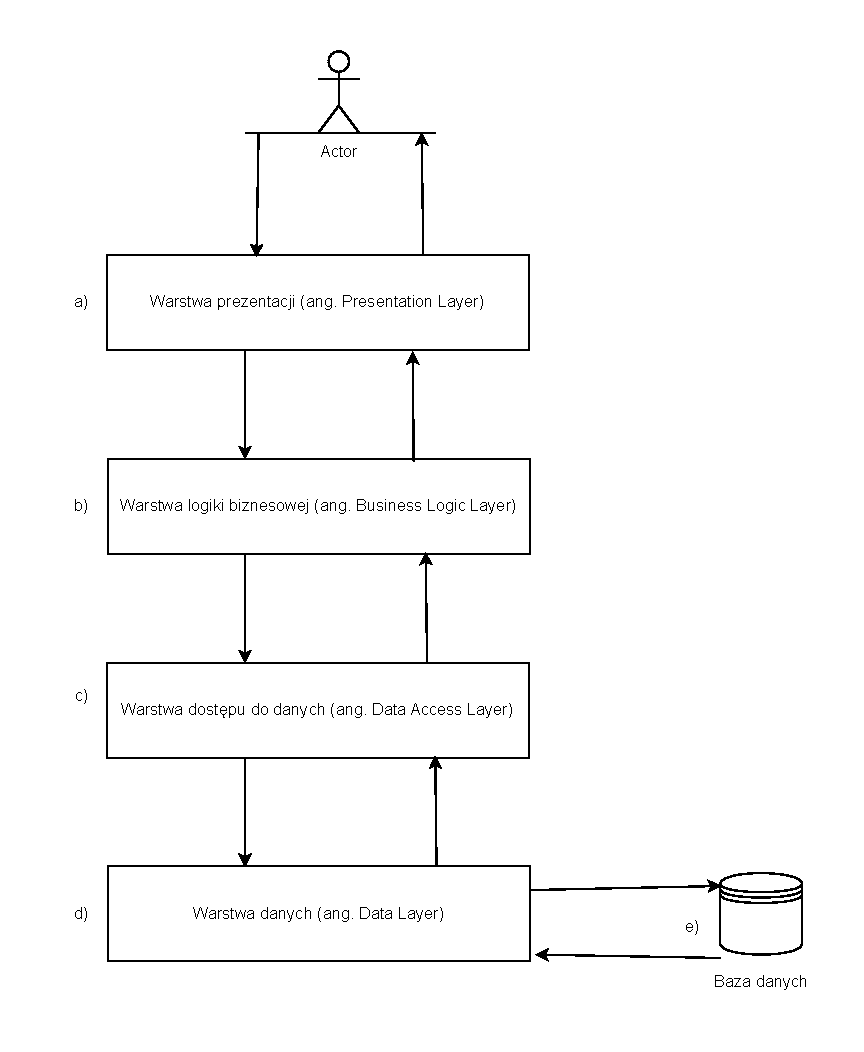
\includegraphics[scale=1]{rys03/diagram_architektury_warstwowej}
    \caption{Ogólny schemat architektury warstwowej}
    \label{fig:n_tier_arch}
\end{figure}

\subsection{Warstwa prezentacji (ang.\ \emph{Presentation Layer})}
Warstwa prezentacji odpowiada za interakcję użytkownika z aplikacją, będąc głównym punktem styku użytkownika z systemem. Na tym poziomie użytkownik wprowadza dane wejściowe, a system zwraca wyniki w formie czytelnej i zrozumiałej. Głównym zadaniem warstwy prezentacji jest renderowanie interfejsu użytkownika oraz obsługa zdarzeń takich jak kliknięcia czy przesunięcia. Odpowiada również za wstępną walidację danych wejściowych, na przykład sprawdzanie, czy wprowadzony adres e-mail ma poprawny format. Przetworzone dane są następnie przekazywane do warstwy logiki biznesowej, gdzie są dalej analizowane i przetwarzane.

Na rysunku \ref{fig:n_tier_arch} warstwa prezentacji jest oznaczona literą \texttt{a)}. W systemie ,,Harmony Home Net,, została zrealizowana za pomocą frameworka Next.js w języku TypeScript. Odpowiada ona za wyświetlanie interfejsu użytkownika, w tym panelu mieszkańca, gdzie użytkownicy mogą przeglądać zgłoszenia techniczne, dokonywać płatności oraz uczestniczyć w głosowaniach. Użycie Next.js umożliwia renderowanie po stronie serwera, co poprawia wydajność aplikacji oraz jej pozycjonowanie w wyszukiwarkach (SEO). Dzięki komponentom wielokrotnego użytku interfejs użytkownika jest spójny wizualnie i funkcjonalnie. 

\subsection{Warstwa logiki biznesowej (ang.\ \emph{Business Logic Layer})}

Warstwa logiki biznesowej pełni kluczową rolę w przetwarzaniu danych wejściowych i realizacji reguł biznesowych. Na tym poziomie dane są analizowane i przetwarzane zgodnie z zasadami określonymi przez specyfikę aplikacji. Główne zadania tej warstwy obejmują koordynację przepływu danych między innymi warstwami oraz obsługę wyjątków, które mogą wystąpić w wyniku błędów na wcześniejszych etapach przetwarzania.

Na rysunku \ref{fig:n_tier_arch} warstwa logiki biznesowej jest oznaczona  literą \texttt{b)}. W~systemie ,,Harmony Home Net,, warstwa ta, oparta na Spring Boot, realizuje procesy biznesowe takie jak autoryzacja użytkowników przy użyciu OAuth 2.0, zarządzanie zgłoszeniami technicznymi oraz integracja z systemami płatności. Warstwa ta komunikuje się z frontendem poprzez REST API, co zapewnia efektywne przetwarzanie żądań i odpowiedzi. Dodatkowo technologia Spring Boot umożliwia implementację skalowalnych i bezpiecznych rozwiązań, co jest kluczowe w przypadku obsługi dużej liczby użytkowników.

\subsection{Warstwa dostępu do danych (ang.\ \emph{Data Access Layer})}

Warstwa dostępu do danych odpowiada za komunikację między logiką biznesową a fizycznym przechowywaniem danych. Jej główną funkcją jest wykonywanie operacji takich jak zapisywanie, odczytywanie, aktualizowanie i usuwanie danych w sposób zoptymalizowany i bezpieczny. Często korzysta się z bibliotek ORM, takich jak Hibernate lub JPA w Javie, które ułatwiają mapowanie danych między bazą a obiektami aplikacji.

Na rysunku \ref{fig:n_tier_arch} warstwa dostępu do danych jest oznaczona literą \texttt{c)}. W systemie ,,Harmony Home Net,, baza danych PostgreSQL została uruchomiona w środowisku Docker. Dzięki zastosowaniu JPA możliwe jest łatwe mapowanie danych między tabelami bazodanowymi a obiektami aplikacji w Javie. Taka implementacja umożliwia optymalizację zapytań i zapewnia wydajność operacji, co jest istotne w przypadku dużej ilości danych przechowywanych w systemie, takich jak zgłoszenia techniczne czy płatności mieszkańców.

\subsection{Warstwa danych (ang.\ \emph{Data Layer})}

Warstwa danych odpowiada za trwałe przechowywanie danych aplikacji w bazach danych. Obejmuje zarządzanie strukturą danych, ich bezpieczeństwem oraz udostępnianie ich innym warstwom w sposób wydajny i zorganizowany. W systemie ,,Harmony Home Net'' wykorzystano bazę danych PostgreSQL, która została wdrożona w kontenerze Docker. 

Na rysunku \ref{fig:n_tier_arch} warstwa danych jest oznaczona literą \texttt{d)}. Dzięki zastosowaniu mapowania ORM dane w bazie są bezpośrednio odwzorowywane na obiekty w aplikacji, co pozwala na wygodniejsze operacje na danych. Mechanizm ORM umożliwia wykonywanie zapytań SQL w sposób abstrakcyjny i bardziej czytelny, co upraszcza implementację i zmniejsza ryzyko błędów.


\section{Struktura bazy danych}

Projektowanie bazy danych to jeden z kluczowych etapów tworzenia systemów informatycznych. W kontekście systemu ,,Harmony Home Net'' zdecydowano się na podejście \emph{Database First}, które polega na zaprojektowaniu struktury bazy danych przed rozpoczęciem implementacji kodu aplikacji. Jest to jedno z dwóch popularnych podejść do projektowania baz danych w aplikacjach, obok \emph{Code First}~\cite{DB_FIRST_VS_CODE_FIRST_1,DB_FIRST_VS_CODE_FIRST_2}.

\subsection{Porównanie podejść Database First i Code First}

Podejście \emph{Code First} zakłada najpierw zaprojektowanie modelu danych w kodzie aplikacji, a następnie generowanie schematu bazy danych na podstawie tego modelu~\cite{CODE_FIRST}. To rozwiązanie charakteryzuje się dużą elastycznością, co pozwala na dynamiczne zmiany w strukturze danych podczas rozwoju aplikacji. Jest ono szczególnie przydatne w projektach, gdzie schemat bazy danych może często ewoluować w odpowiedzi na zmieniające się wymagania biznesowe. Jednakże, z uwagi na brak wstępnego schematu, podejście \emph{Code First} może być trudniejsze do utrzymania w dużych projektach, w których schemat danych jest złożony i wymaga precyzyjnej kontroli.

Z kolei podejście \emph{Database First} polega na wcześniejszym zaprojektowaniu schematu bazy danych, a następnie wygenerowaniu modelu aplikacji na jego podstawie. Jest to podejście bardziej tradycyjne, które umożliwia dokładne zdefiniowanie struktury danych jeszcze przed rozpoczęciem kodowania aplikacji~\cite{DB_FIRST}. Taka metodologia daje większą przewidywalność i precyzję, co jest istotne w systemach o wysokim stopniu zależności od integralności danych. Dodatkowo, podejście to pozwala na pełne wykorzystanie możliwości narzędzi ORM, takich jak JPA, ponieważ bazuje na uprzednio zaprojektowanym schemacie.

\subsection{Wyboru podejścia Database First}

W systemie „Harmony Home Net” zdecydowano się na podejście \emph{Database First} z kilku kluczowych powodów:

\begin{itemize}
    \item \textbf{Centralna rola bazy danych} -- baza danych pełni kluczową funkcję w systemie, przechowując informacje o użytkownikach, lokalach, zgłoszeniach technicznych oraz płatnościach. Precyzyjne zaprojektowanie jej struktury na etapie początkowym pozwoliło na lepsze zrozumienie relacji między danymi i~ich hierarchii.
    \item \textbf{Integracja z narzędziami ORM} -- dzięki wykorzystaniu podejścia \emph{Database First}, istniejące narzędzia ORM, takie jak JPA (Java Persistence API), mogły zostać bezproblemowo dostosowane do uprzednio przygotowanego schematu bazy danych, co uprościło implementację i~zmniejszyło ryzyko błędów.
    \item \textbf{Zgodność z wymaganiami aplikacji} -- rozpoczęcie od projektowania bazy danych zapewniło uzyskanie zgodności struktury danych z wymaganiami funkcjonalnymi i niefunkcjonalnymi. Umożliwiło również identyfikację potencjalnych problemów na wczesnym etapie prac.
    \item \textbf{Bezpieczeństwo i integralność danych} -- projektując bazę danych jako pierwszą można było od razu uwzględnić mechanizmy zabezpieczeń, takie jak klucze główne, obce oraz indeksy. Zminimalizowało to ryzyko wystąpienia niespójności danych w trakcie działania systemu.
\end{itemize}

\subsection{Opis struktury bazy danych}

Strukturę bazy danych w systemie „Harmony Home Net” zaprojektowano z uwzględnieniem wymagań funkcjonalnych i niefunkcjonalnych aplikacji. Schemat bazy danych podzielono na warstwę konceptualną (rysunek \ref{fig:ebok_db_concept}) oraz fizyczną (rysunek \ref{fig:ebok_db_physical}), co umożliwiło dokładne odwzorowanie relacji pomiędzy danymi oraz optymalizację ich przechowywania.

\begin{figure}[ht]
    \centering
    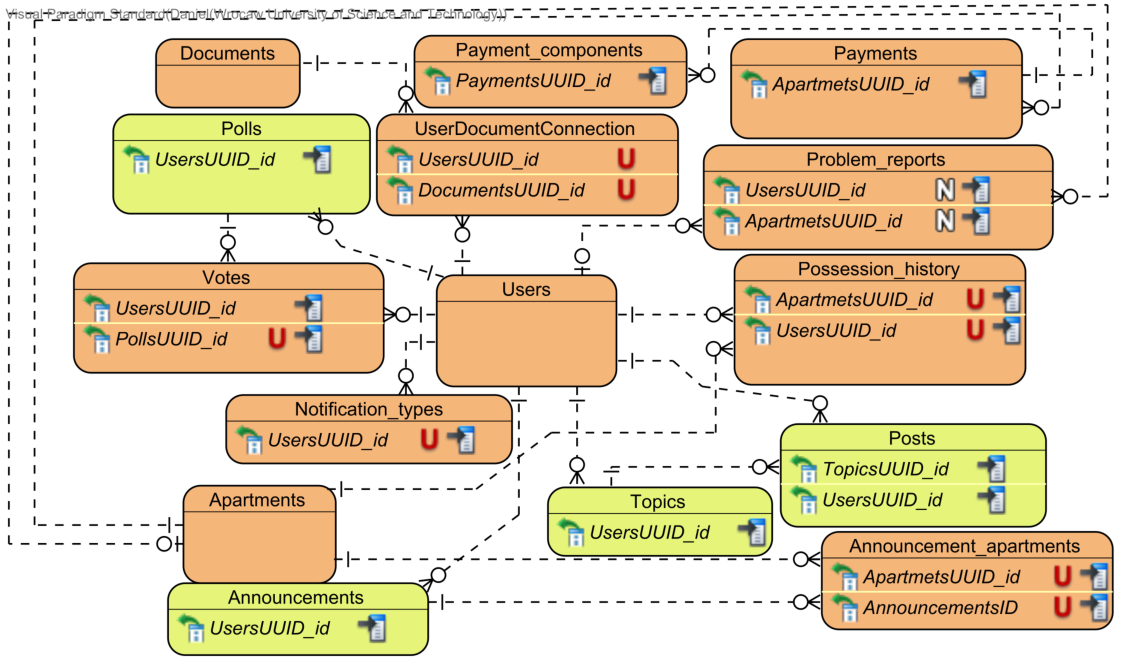
\includegraphics[width=.9\linewidth]{rys03/ebok_db_concept}
    \caption{Schemat konceptualny bazy danych systemu}
    \label{fig:ebok_db_concept}
\end{figure}

\begin{figure}[ht]
    \centering
    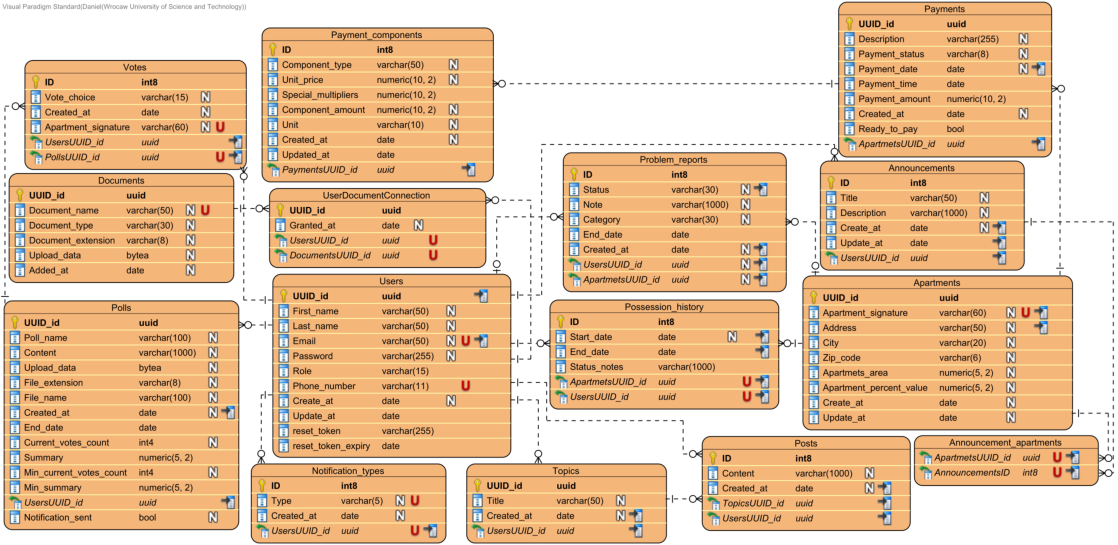
\includegraphics[width=1\linewidth]{rys03/ebok_db_physical}
    \caption{Schemat fizyczny bazy danych systemu}
    \label{fig:ebok_db_physical}
\end{figure}

\subsubsection{Opis tabel}

Poniżej szczegółowo opisano wszystkie tabele w bazie danych:

\begin{itemize}
    \item \textbf{Tabela \texttt{Users}:}
    Przechowuje dane o użytkownikach, takie jak:
    \begin{itemize}
        \item \texttt{FirstName} i \texttt{LastName} -- imię i nazwisko użytkownika,
        \item \texttt{Email} -- unikalny adres e-mail,
        \item \texttt{Password} -- zaszyfrowane hasło,
        \item \texttt{Role} -- rola w systemie (np. właściciel, pracownik, administrator),
        \item \texttt{CreateAt} i \texttt{UpdateAt} -- daty utworzenia i ostatniej modyfikacji rekordu.
    \end{itemize}
    Klucz główny \texttt{UUID} jest wykorzystywany jako klucz obcy w wielu innych tabelach, zapewniając spójność relacji.

    \item \textbf{Tabela \texttt{Apartments}:}
    Zawiera szczegółowe dane o lokalach:
    \begin{itemize}
        \item \texttt{ApartmentSignature} -- unikalny identyfikator lokalu,
        \item \texttt{Address}, \texttt{City} i \texttt{ZipCode} -- adres lokalu,
        \item \texttt{ApartmentArea} -- powierzchnia,
        \item \texttt{ApartmentPercentValue} -- udział procentowy w nieruchomości wspólnej.
    \end{itemize}
    Powiązana z użytkownikami poprzez klucz obcy \texttt{UsersUUID}.
    
    \item \textbf{Tabela \texttt{Payments}:}
    Rejestruje dane o płatnościach:
    \begin{itemize}
        \item \texttt{Description}, \texttt{PaymentStatus}, \texttt{PaymentDate}, \texttt{PaymentAmount},
        \item \texttt{ReadyToPay} -- znacznik stanu płatności.
    \end{itemize}

    \item \textbf{Tabela \texttt{PaymentComponent}:}
    Szczegółowo opisuje składniki płatności, co pozwala na większą elastyczność w obliczaniu należności. Przechowuje informacje takie jak:
    \begin{itemize}
        \item \texttt{ComponentType} -- typ składnika płatności (np. czynsz, media, fundusz remontowy),
        \item \texttt{UnitPrice} i \texttt{ComponentAmount} -- cena jednostkowa i łączna kwota dla składnika,
        \item \texttt{SpecialMultipliers} -- specjalne mnożniki stosowane w obliczeniach (np. liczba osób, powierzchnia lokalu),
        \item \texttt{Unit} -- jednostka składnika (np. m\textsuperscript{2}, sztuki).
    \end{itemize}
    Tabela jest powiązana z tabelą \texttt{Payments} poprzez klucz obcy \texttt{PaymentsUUID}.

    \item \textbf{Tabela \texttt{ProblemReports}:}
    Zawiera zgłoszenia techniczne dotyczące lokali:
    \begin{itemize}
        \item \texttt{Status}, \texttt{Category}, \texttt{Note} -- szczegóły zgłoszenia,
        \item Klucze obce \texttt{UsersUUID} i \texttt{ApartmentsUUID}.
    \end{itemize}

    \item \textbf{Tabela \texttt{Polls} i \texttt{Votes}:}
    Obsługuje głosowania:
    \begin{itemize}
        \item Tabela \texttt{Polls} zawiera dane głosowań, a \texttt{Votes} przechowuje głosy użytkowników,
        \item Wprowadzono ograniczenie unikalności głosów w relacji \texttt{pollId} oraz \texttt{apartmentSignature}.
    \end{itemize}

    \item \textbf{Tabela \texttt{Documents} i \texttt{UserDocumentConnection}:}
    \texttt{UserDocumentConnection} pełni rolę łącznika w relacji wiele do wielu między \texttt{Users} a \texttt{Documents}. Tabela \texttt{Documents} przechowuje informacje o plikach, takie jak nazwa, typ, treść (\texttt{UploadData}) oraz data dodania.
    
    \item \textbf{Tabela \texttt{Announcements} i \texttt{AnnouncementApartment}:}
    \texttt{Announcements} przechowuje ogłoszenia, a \texttt{AnnouncementApartment} pełni rolę tabeli łącznikowej w relacji wiele do wielu między \texttt{Announcements} a \texttt{Apartments}.

    \item \textbf{Tabela \texttt{NotificationTypes}:}
    Przechowuje różne typy powiadomień i ich relacje z użytkownikami. Zdefiniowano ograniczenie unikalności, które uniemożliwia przypisanie tego samego typu powiadomienia temu samemu użytkownikowi wielokrotnie.

    \item \textbf{Tabela \texttt{PossessionHistory}:}
    Rejestruje historię przypisania użytkowników do lokali:
    \begin{itemize}
        \item \texttt{StartDate} i \texttt{EndDate} -- okres użytkowania lokalu,
        \item Klucze obce \texttt{ApartmentsUUID} i \texttt{UsersUUID}.
        \item Zastosowano ograniczenie unikalności relacji między \texttt{userId} a \texttt{apartmentId}.
    \end{itemize}
\end{itemize}

\subsubsection{Podział tabel na pakiety}

W implementacji kodu wszystkie tabele zostały podzielone na dwa logiczne pakiety:
\begin{itemize}
    \item \textbf{Pakiet \texttt{sideTables}:} Obejmuje tabele pomocnicze, które pełnią rolę łączników w relacjach wiele do wielu. Należą do niego:
    \begin{itemize}
        \item \texttt{UserDocumentConnection},
        \item \texttt{PossessionHistory},
        \item \texttt{AnnouncementApartment}.
    \end{itemize}

    \item \textbf{Pakiet \texttt{mainTables}:} Obejmuje główne tabele przechowujące kluczowe dane systemu, takie jak:
    \begin{itemize}
        \item \texttt{Users},
        \item \texttt{Apartments},
        \item \texttt{Payments},
        \item \texttt{PaymentComponent},
        \item \texttt{ProblemReports},
        \item \texttt{Polls},
        \item \texttt{Votes},
        \item \texttt{Documents},
        \item \texttt{Announcements},
        \item \texttt{NotificationTypes}.
    \end{itemize}
\end{itemize}

Podział tabel na dwa pakiety zapewnia przejrzystość struktury kodu, łatwość zarządzania relacjami między encjami oraz ułatwia przyszłą rozbudowę systemu.


\subsection{Relacje i integralność danych}

Relacje między tabelami zostały szczegółowo odwzorowane za pomocą kluczy głównych i obcych, co umożliwia utrzymanie integralności danych oraz łatwe zarządzanie połączeniami między różnymi elementami bazy. Na przykład, tabela \texttt{Problem\_reports} zawiera klucze obce do tabel \texttt{Users} i \texttt{Apartments}, co pozwala na przypisanie zgłoszeń technicznych zarówno do konkretnego użytkownika, jak i lokalu. Analogicznie, tabela \texttt{Payments} jest powiązana z tabelą \texttt{Apartments}, co zapewnia pełną kontrolę nad płatnościami przypisanymi do danych lokali.

\subsection{Mechanizmy optymalizacyjne}

W celu poprawy wydajności bazy danych zastosowano następujące mechanizmy:
\begin{itemize}
    \item \textbf{Indeksy} -- kluczowe kolumny, takie jak \texttt{UUID}, zostały zaindeksowane w celu przyspieszenia operacji wyszukiwania i sortowania.
    \item \textbf{Mapowanie ORM} -- baza danych została zintegrowana z aplikacją za pomocą narzędzia JPA (Java Persistence API), co umożliwia bezpośrednie mapowanie tabel na obiekty w kodzie aplikacji. Dzięki temu operacje CRUD (Create, Read, Update, Delete) mogą być realizowane w sposób wygodny i abstrakcyjny, bez konieczności pisania zapytań SQL.
    \item \textbf{Konteneryzacja} -- PostgreSQL działa w środowisku Docker, co zapewnia łatwość zarządzania i możliwość skalowania systemu w zależności od obciążenia.
		\item \textbf{Ograniczenia unikalności (ang. Unique Constraint)} -- w tabelach takich jak \texttt{Votes}, \texttt{PossessionHistory}, \texttt{NotificationTypes}, oraz \texttt{AnnouncementApartment} zastosowano ograniczenia unikalności (\texttt{UniqueConstraints}), co zapobiega wprowadzaniu niepożądanych duplikatów w relacjach wiele do wielu.
\end{itemize}

\subsection{Podsumowanie}

Struktura bazy danych systemu \textbf{Harmony Home Net} została zaprojektowana w sposób umożliwiający jej skalowalność, wydajność oraz łatwość integracji z innymi komponentami aplikacji. Podejście \emph{Database First} okazało się optymalnym wyborem, zapewniając precyzyjne odwzorowanie wymagań biznesowych i technicznych systemu. Schematy konceptualny (rysunek \ref{fig:ebok_db_concept}) i fizyczny (rysunek \ref{fig:ebok_db_physical}) ilustrują relacje pomiędzy tabelami, które stanowią podstawę spójnego i efektywnego zarządzania danymi.

\section{Bezpieczeństwo, uwierzytelnianie i autoryzacja w aplikacji}


\subsection{Wprowadzenie do mechanizmów bezpieczeństwa}

Sekcja dotycząca bezpieczeństwa opisuje mechanizmy zastosowane w systemie „Harmony Home Net” w celu zapewnienia ochrony danych użytkowników oraz bezpiecznego dostępu do zasobów. W ramach tej części pracy przedstawione zostały szczegóły implementacji konfiguracji bezpieczeństwa opartej na Spring Security, wykorzystanie tokenów JWT oraz \emph{OAuth 2.0 Resource Server} jako mechanizmów uwierzytelniania i autoryzacji.

W szczególności omówiono rolę \emph{OAuth 2.0 Resource Server} w weryfikacji tokenów dostępu generowanych w ramach sesji użytkownika. Mechanizm ten umożliwia bezpieczne zarządzanie dostępem do zasobów oraz bezstanowe uwierzytelnianie użytkowników, eliminując konieczność utrzymywania sesji po stronie serwera.

W tej sekcji można znaleźć:

\begin{itemize}
    \item \textbf{Wprowadzenie do mechanizmów bezpieczeństwa} -- Omówienie kluczowych elementów konfiguracji, takich jak filtry bezpieczeństwa (\emph{SecurityFilterChain}), zarządzanie sesjami w trybie bezstanowym oraz zabezpieczenie API za pomocą tokenów JWT i \emph{OAuth 2.0 Resource Server}. W tej części przedstawiono również znaczenie \texttt{JwtAuthenticationConverter} i jego rolę w integracji z mechanizmami Spring Security.

    \item \textbf{Proces logowania} -- Szczegółowy opis procesu logowania z wykorzystaniem nazw użytkowników, haseł oraz generowania tokenów JWT. Proces uwierzytelniania użytkowników opisano w oparciu o klasę \texttt{UserInfoManagerConfig}, która integruje bazę danych z mechanizmami uwierzytelniania w Spring Security.

    \item \textbf{Zarządzanie tokenami JWT i autoryzacji użytkowników} -- Szczegółowy opis sposobu generowania i weryfikacji tokenów JWT. Proces ten obejmuje również schemat związany z uwierzytelnianiem użytkowników przy użyciu \emph{OAuth 2.0 Resource Server}. Omówiono mechanizmy sprawdzania poprawności i wykrywania wygasłych lub nieautoryzowanych tokenów, a także kluczową rolę klasy \texttt{JwtAccessTokenFilter}, która weryfikuje tokeny w żądaniach HTTP.

    \item \textbf{Zarządzanie czarną listą tokenów} -- Implementacja usługi \texttt{TokenBlacklistService}, która pozwala na unieważnianie tokenów w momencie wylogowania użytkownika. Dzięki temu użytkownicy mogą zostać natychmiast wylogowani, a sesje mogą być anulowane w przypadku wykrycia naruszeń bezpieczeństwa. Usługa obejmuje również harmonogram automatycznego usuwania wygasłych tokenów z czarnej listy, co zwiększa wydajność systemu.

    \item \textbf{Mechanizmy resetowania hasła} -- Konfiguracja specjalnego łańcucha filtrów bezpieczeństwa dedykowanego resetowaniu hasła, który umożliwia różnicowanie poziomów dostępu na podstawie ścieżek. Mechanizm ten obsługuje żądania związane z resetowaniem hasła, przy zachowaniu odpowiedniego poziomu bezpieczeństwa dla publicznych punktów końcowych.

\end{itemize}



\subsection{Konfiguracja łańcucha filtrów bezpieczeństwa}

Łańcuch filtrów bezpieczeństwa (\emph{Security Filter Chain}) odgrywa kluczową rolę w zapewnieniu ochrony aplikacji. W systemie „Harmony Home Net” został on skonfigurowany przy użyciu klasy \texttt{SecurityConfig}, która definiuje różne ścieżki żądań oraz odpowiadające im mechanizmy uwierzytelniania i autoryzacji. Każda ścieżka obsługiwana jest przez dedykowany łańcuch filtrów, co umożliwia elastyczne zarządzanie poziomem bezpieczeństwa.

W konfiguracji wykorzystano mechanizm \texttt{JwtAuthenticationConverter}, który umożliwia niestandardowe przekształcanie tokenów JWT na obiekty \texttt{Authentication}, dodając autoryzacje na podstawie zawartości tokenu. Dzięki temu aplikacja może elastycznie zarządzać dostępem użytkowników na podstawie przypisanych im ról lub innych atrybutów zawartych w tokenie JWT.

Kluczowym elementem konfiguracji jest również zastosowanie adnotacji \texttt{@Order}. Każdy łańcuch filtrów posiada określoną kolejność, która decyduje o tym, w jakiej sekwencji będą przetwarzane żądania. Dzięki temu można precyzyjnie kontrolować, które mechanizmy mają priorytet w przetwarzaniu poszczególnych ścieżek. Niewłaściwe ustawienie kolejności mogłoby spowodować nieprawidłowe działanie zabezpieczeń.

W systemie zaimplementowano cztery główne łańcuchy filtrów:
\begin{itemize}
    \item \textbf{Łańcuch obsługi resetowania hasła} -- scieżki \texttt{/auth/forgot-password} i \texttt{/auth/reset-password} są publicznie dostępne bez konieczności uwierzytelniania (\texttt{@Order(1)}).
    \item \textbf{Łańcuch logowania} -- obsługuje ścieżkę \texttt{/auth/login}, zapewniając uwierzytelnianie użytkownika przy użyciu nazw użytkowników i haseł (\texttt{@Order(2)}).
    \item \textbf{Łańcuch API} -- chroni wszystkie ścieżki API zaczynające się od \texttt{/api/v1/}, wymagając tokenu JWT do autoryzacji (\texttt{@Order(3)}).
    \item \textbf{Łańcuch wylogowania} -- obsługuje ścieżkę \texttt{/logout}, umożliwiając wylogowanie użytkownika i unieważnienie tokenu JWT (\texttt{@Order(4)}).
\end{itemize}

Każdy z łańcuchów został skonfigurowany jako komponent Spring Bean, dzięki czemu można elastycznie dostosowywać ustawienia w zależności od potrzeb. Poniżej przedstawiono pełny kod konfiguracji:

\begin{lstlisting}[language=Java, caption=Pełna konfiguracja łańcucha filtrów bezpieczeństwa]
@Configuration
@EnableWebSecurity
@EnableMethodSecurity
@RequiredArgsConstructor
@Import(JwtConfig.class)
public class SecurityConfig {

    private final UserInfoManagerConfig userInfoManagerConfig;
    private final RSAKeyRecord rsaKeyRecord;
    private final JwtTokenUtils jwtTokenUtils;
    private final TokenBlacklistService tokenBlacklistService;

    @Order(1)
    @Bean
    public SecurityFilterChain forgotPasswordSecurityFilterChain(HttpSecurity httpSecurity) throws Exception {
        return httpSecurity
                .securityMatcher(new OrRequestMatcher(
                        new AntPathRequestMatcher("/auth/forgot-password"),
                        new AntPathRequestMatcher("/auth/reset-password")
                ))
                .csrf(AbstractHttpConfigurer::disable)
                .authorizeHttpRequests(auth -> auth.anyRequest().permitAll())
                .sessionManagement(session -> session.sessionCreationPolicy(SessionCreationPolicy.STATELESS))
                .cors(withDefaults())
                .build();
    }

    @Order(2)
    @Bean
    public SecurityFilterChain loginSecurityFilterChain(HttpSecurity http) throws Exception {
        return http
                .securityMatcher(new AntPathRequestMatcher("/auth/login"))
                .csrf(AbstractHttpConfigurer::disable)
                .authorizeHttpRequests(auth -> auth.anyRequest().authenticated())
                .userDetailsService(userInfoManagerConfig)
                .sessionManagement(session -> session.sessionCreationPolicy(SessionCreationPolicy.STATELESS))
                .httpBasic(withDefaults())
                .cors(withDefaults())
                .build();
    }

    @Order(3)
    @Bean
    public SecurityFilterChain apiSecurityFilterChain(HttpSecurity http) throws Exception {
        return http
                .securityMatcher(new AntPathRequestMatcher("/api/v1/**"))
                .csrf(AbstractHttpConfigurer::disable)
                .authorizeHttpRequests(auth -> auth.anyRequest().authenticated())
                .oauth2ResourceServer(oauth2 -> oauth2
                        .jwt(jwt -> jwt.jwtAuthenticationConverter(jwtAuthenticationConverter()))
                )
                .sessionManagement(session -> session.sessionCreationPolicy(SessionCreationPolicy.STATELESS))
                .addFilterBefore(new JwtAccessTokenFilter(rsaKeyRecord, jwtTokenUtils, tokenBlacklistService), UsernamePasswordAuthenticationFilter.class)
                .cors(withDefaults())
                .build();
    }

    @Order(4)
    @Bean
    public SecurityFilterChain logoutSecurityFilterChain(HttpSecurity httpSecurity) throws Exception {
        return httpSecurity
                .securityMatcher(new AntPathRequestMatcher("/logout"))
                .csrf(AbstractHttpConfigurer::disable)
                .authorizeHttpRequests(auth -> auth.anyRequest().authenticated())
                .logout(logout -> logout
                        .logoutUrl("/logout")
                        .logoutSuccessHandler((request, response, authentication) -> {
                            String token = request.getHeader("Authorization").replace("Bearer ", "");
                            tokenBlacklistService.blacklistToken(token);
                            SecurityContextHolder.clearContext();
                        })
                )
                .cors(withDefaults())
                .build();
    }

    @Bean
    public JwtAuthenticationConverter jwtAuthenticationConverter() {
        JwtAuthenticationConverter converter = new JwtAuthenticationConverter();
        converter.setJwtGrantedAuthoritiesConverter(jwt -> {
            List<GrantedAuthority> authorities = new ArrayList<>();
            String role = jwt.getClaimAsString("role");
            if (role != null) {
                authorities.add(new SimpleGrantedAuthority(role));
            }
            return authorities;
        });
        return converter;
    }
}
\end{lstlisting}

---

Dzięki tej konfiguracji system:
\begin{itemize}
    \item Rozdziela odpowiedzialność za różne ścieżki żądań, pozwalając na precyzyjne zarządzanie dostępem.
    \item Wykorzystuje \texttt{JwtAuthenticationConverter} do niestandardowego zarządzania autoryzacją na podstawie zawartości tokenu JWT.
    \item Umożliwia bezstanowe zarządzanie sesjami za pomocą tokenów JWT.
    \item Zachowuje odpowiednią kolejność przetwarzania żądań dzięki zastosowaniu adnotacji \texttt{@Order}.
\end{itemize}

\subsection{Proces logowania}

Mechanizm logowania w systemie „Harmony Home Net” został zaprojektowany w oparciu o Spring Security i tokeny JWT. Poniżej przedstawiono szczegółowy opis procesu logowania, krok po kroku, na podstawie schematu zaprezentowanego na rysunku \ref{fig:ebok_db_concept}.

\begin{figure}[ht]
    \centering
    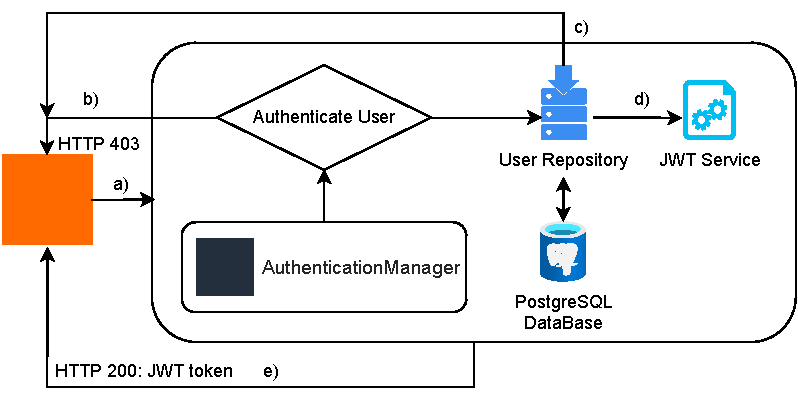
\includegraphics[width=.9\linewidth]{rys03/proces_logowania}
    \caption{Schemat działania procesu logowania w systemie~\cite{JWToauth}}
    \label{fig:ebok_db_concept}
\end{figure}

Proces logowania składa się z następujących kroków, oznaczonych literami \textbf{a}–\textbf{e} na schemacie:

\begin{enumerate}
    \item \textbf{Przesłanie danych logowania \texttt{a)}} -- Użytkownik wysyła żądanie HTTP \texttt{POST} na endpoint \texttt{/auth/login}, dostarczając swoje dane logowania, takie jak nazwa użytkownika i hasło. 
		
    \item \textbf{Uwierzytelnienie użytkownika przez \texttt{AuthenticationManager} \texttt{b)}} -- \texttt{AuthenticationManager} to kluczowy komponent Spring Security, który weryfikuje dane logowania. W pierwszym kroku proces uwierzytelniania odbywa się za pomocą dostarczonej nazwy użytkownika i hasła.

    \item \textbf{Sprawdzenie danych w repozytorium użytkowników \texttt{c)}} -- \texttt{AuthenticationManager} deleguje żądanie do repozytorium użytkowników (\texttt{UserRepository}), które weryfikuje, czy użytkownik o podanym loginie istnieje w systemie. W tym celu wykorzystywana jest klasa \texttt{UserInfoManagerConfig}, która implementuje interfejs \texttt{UserDetailsService}. Jeśli użytkownik nie zostanie znaleziony lub dane logowania są niepoprawne, proces logowania kończy się niepowodzeniem i zwracany jest status \texttt{HTTP 403}.

    \item \textbf{Generowanie tokenu JWT \texttt{d)}} -- Jeśli dane logowania są poprawne, na podstawie informacji o użytkowniku generowany jest token JWT za pomocą usługi \texttt{JwtService}. Token zawiera zaszyfrowane informacje, takie jak identyfikator użytkownika, rola w systemie oraz data wygaśnięcia. Klucze RSA zapewniają bezpieczeństwo tokenu.

    \item \textbf{Zwrócenie tokenu JWT w odpowiedzi \texttt{e)}} -- Token JWT jest przesyłany do użytkownika w odpowiedzi HTTP \texttt{200}. Użytkownik przechowuje token lokalnie (np. w pamięci przeglądarki lub w \emph{localStorage}), aby używać go do autoryzacji kolejnych żądań do API.
\end{enumerate}

W szczególności klasa \texttt{UserInfoManagerConfig}, wykorzystywana w kroku \texttt{c)}, jest odpowiedzialna za weryfikację istnienia użytkownika w bazie danych oraz dostarczenie szczegółów użytkownika wymaganych przez mechanizm uwierzytelniania. Kod klasy przedstawiono poniżej:

\begin{lstlisting}[language=Java, caption=Klasa \texttt{UserInfoManagerConfig} odpowiedzialna za zarządzanie użytkownikami]
package bwp.hhn.backend.harmonyhomenetlogic.configuration.security;

import bwp.hhn.backend.harmonyhomenetlogic.repository.mainTables.UserRepository;
import lombok.RequiredArgsConstructor;
import org.springframework.security.core.userdetails.UserDetails;
import org.springframework.security.core.userdetails.UserDetailsService;
import org.springframework.security.core.userdetails.UsernameNotFoundException;
import org.springframework.stereotype.Service;

@Service
@RequiredArgsConstructor
public class UserInfoManagerConfig implements UserDetailsService {

    private final UserRepository userRepository;

    @Override
    public UserDetails loadUserByUsername(String username) throws UsernameNotFoundException {
        return userRepository.findByEmail(username)
                .orElseThrow(() -> new UsernameNotFoundException("User not found"));
    }
}
\end{lstlisting}

Kluczowe funkcje tej klasy:
\begin{itemize}
    \item \textbf{Implementacja metody \texttt{loadUserByUsername}:} Weryfikuje istnienie użytkownika w bazie danych na podstawie adresu e-mail.
    \item \textbf{Obsługa wyjątków:} W przypadku, gdy użytkownik nie zostanie znaleziony, rzucany jest wyjątek \texttt{UsernameNotFoundException}, który kończy proces logowania.
    \item \textbf{Repozytorium \texttt{UserRepository}:} Umożliwia dostęp do bazy danych w celu wyszukiwania użytkowników.
\end{itemize}

Mechanizm logowania zapewnia bezpieczną i bezstanową autoryzację użytkowników, minimalizując ryzyko naruszenia danych i nieuprawnionego dostępu.

\subsection{Zarządzanie tokenami JWT i autoryzacja użytkowników}

Zarządzanie tokenami JWT w systemie „Harmony Home Net” opiera się na zaawansowanych mechanizmach walidacji i autoryzacji, integrując je z frameworkiem Spring Security. Schemat ilustrujący proces dostępu do zasobów systemu został przedstawiony na rysunku \ref{fig:resource_access_flow}.

\begin{figure}[ht]
    \centering
    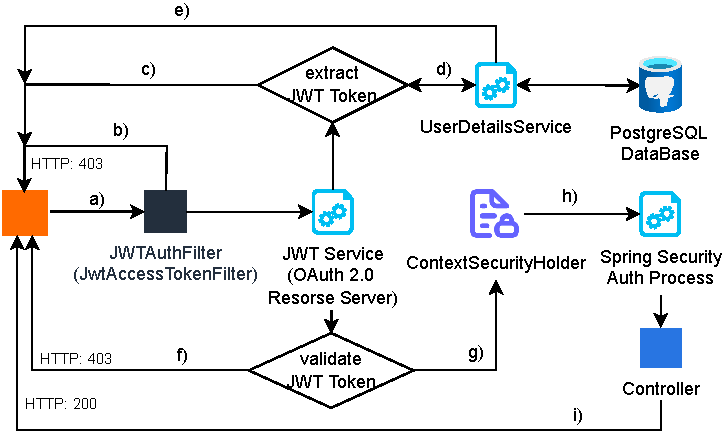
\includegraphics[width=.9\linewidth]{rys03/Diagram_dotępu_do_zasobów_systemu}
    \caption{Diagram zarządzania tokenami JWT i autoryzacji użytkowników~\cite{JWToauth}}
    \label{fig:resource_access_flow}
\end{figure}

Proces składa się z następujących kroków, oznaczonych literami \textbf{a}–\textbf{i} na schemacie:

\begin{itemize}
    \item \textbf{Przesłanie żądania przez użytkownika \texttt{a)}} -- użytkownik wysyła żądanie HTTP do usługi API z dołączonym tokenem JWT w nagłówku \texttt{Authorization}.
    
    \item \textbf{Przechwycenie żądania przez \texttt{JwtAccessTokenFilter} \texttt{b)}} -- niestandardowy filtr \texttt{JwtAccessTokenFilter}, zintegrowany z \texttt{SecurityFilterChain}, przechwytuje żądanie i analizuje token JWT. Jeśli token jest nieobecny lub niepoprawny, zwracana jest odpowiedź z kodem HTTP \texttt{403}.
    
    \item \textbf{Ekstrakcja danych z tokenu JWT przez \texttt{Jwt Service / OAuth 2.0 Resource Server} \texttt{c)}} -- w przypadku obecności tokenu JWT, usługa \texttt{Jwt Service}, korzystająca z mechanizmu \emph{OAuth 2.0 Resource Server}, jest wywoływana w celu ekstrakcji adresu e-mail użytkownika (\texttt{userEmail}). Jeśli dane użytkownika nie mogą zostać odczytane lub token jest nieprawidłowy, zwracany jest status HTTP \texttt{403}.

    \item \textbf{Sprawdzenie użytkownika w bazie danych \texttt{d)}} -- Wyodrębniony adres e-mail użytkownika jest wykorzystywany do zapytania w bazie danych za pomocą \texttt{UserDetailsService}. Jeśli użytkownik nie istnieje w bazie, zwracana jest odpowiedź z kodem HTTP \texttt{403}.
    
    \item \textbf{Walidacja tokenu JWT \texttt{e)}} -- token JWT jest weryfikowany pod kątem poprawności oraz daty ważności. Jeśli token wygasł, zwracana jest odpowiedź HTTP \texttt{403}.
    
    \item \textbf{Utworzenie obiektu \texttt{UsernamePasswordAuthenticationToken} \texttt{f)}} -- jeśli token JWT jest ważny, informacje o użytkowniku są przetwarzane w obiekt \texttt{UsernamePasswordAuthenticationToken}, który następnie jest przechowywany w \texttt{SecurityContextHolder}.
    
    \item \textbf{Autoryzacja przez Spring Security \texttt{g)}} -- mechanizm autoryzacji Spring Security jest automatycznie wywoływany, aby sprawdzić, czy użytkownik ma odpowiednie uprawnienia do dostępu do zasobów.
    
    \item \textbf{Przekazanie żądania do kontrolera \texttt{h)}} -- po pomyślnym uwierzytelnieniu i autoryzacji żądanie jest kierowane do odpowiedniego kontrolera, który obsługuje dalsze przetwarzanie.
    
    \item \textbf{Zwrócenie odpowiedzi \texttt{i)}} -- po przetworzeniu żądania kontroler zwraca odpowiedź JSON z kodem HTTP \texttt{200}.
\end{itemize}

Kluczowym elementem procesu zarządzania tokenami JWT jest klasa \texttt{JwtAccessTokenFilter}, której zadaniem jest przechwytywanie i weryfikacja tokenów JWT w żądaniach HTTP. Kod tej klasy przedstawiono poniżej:

\begin{lstlisting}[language=Java, caption=Kod niestandardowego filtra \texttt{JwtAccessTokenFilter}]
@RequiredArgsConstructor
public class JwtAccessTokenFilter extends OncePerRequestFilter {

    private final RSAKeyRecord rsaKeyRecord;
    private final JwtTokenUtils jwtTokenUtils;
    private final TokenBlacklistService tokenBlacklistService;

    @Override
    protected void doFilterInternal(@NonNull HttpServletRequest request, 
                                    @NonNull HttpServletResponse response, 
                                    @NonNull FilterChain filterChain) 
            throws ServletException, IOException {

        final String authHeader = request.getHeader(HttpHeaders.AUTHORIZATION);

        if (authHeader == null || !authHeader.startsWith(TokenType.Bearer.name())) {
            filterChain.doFilter(request, response);
            return;
        }

        final String token = authHeader.substring(7);

        if (tokenBlacklistService.isTokenBlacklisted(token)) {
            response.setStatus(HttpStatus.UNAUTHORIZED.value());
            response.getWriter().write("Token is blacklisted");
            return;
        }

        JwtDecoder jwtDecoder = NimbusJwtDecoder.withPublicKey(rsaKeyRecord.publicKey()).build();
        Jwt jwtToken = jwtDecoder.decode(token);

        String userName = jwtTokenUtils.getUserName(jwtToken);

        if (userName != null && SecurityContextHolder.getContext().getAuthentication() == null) {
            UserDetails userDetails = jwtTokenUtils.userDetails(userName);

            if (jwtTokenUtils.isTokenValid(jwtToken, userDetails)) {
                UsernamePasswordAuthenticationToken authToken = new UsernamePasswordAuthenticationToken(
                        userDetails, null, userDetails.getAuthorities());
                authToken.setDetails(new WebAuthenticationDetailsSource().buildDetails(request));
                SecurityContextHolder.getContext().setAuthentication(authToken);
            }
        }
        filterChain.doFilter(request, response);
    }
}
\end{lstlisting}

Opis działania klasy:

\begin{itemize}
    \item Klasa \texttt{JwtAccessTokenFilter} dziedziczy po \texttt{OncePerRequestFilter}, dzięki czemu jest wywoływana raz dla każdego żądania.
    \item Weryfikacja nagłówka \texttt{Authorization} zapewnia, że token JWT jest obecny i poprawny.
    \item Tokeny znajdujące się na czarnej liście są odrzucane z kodem HTTP \texttt{401}.
    \item Token JWT jest dekodowany za pomocą klucza publicznego RSA, a dane użytkownika są odczytywane i weryfikowane.
    \item Po pomyślnej weryfikacji dane użytkownika są zapisywane w \texttt{SecurityContextHolder}, umożliwiając dalszy proces autoryzacji.
\end{itemize}


Klasa \texttt{JwtConfig} zapewnia konfigurację mechanizmów dekodowania i kodowania tokenów JWT przy użyciu kluczy RSA. Kod klasy:

\begin{lstlisting}[language=Java, caption=Klasa \texttt{JwtConfig}]
@Configuration
public class JwtConfig {

    private final RSAKeyRecord rsaKeyRecord;

    public JwtConfig(RSAKeyRecord rsaKeyRecord) {
        this.rsaKeyRecord = rsaKeyRecord;
    }

    @Bean
    public JwtDecoder jwtDecoder() {
        return NimbusJwtDecoder.withPublicKey(rsaKeyRecord.publicKey()).build();
    }

    @Bean
    public JwtEncoder jwtEncoder() {
        JWK jwk = new RSAKey.Builder(rsaKeyRecord.publicKey())
                           .privateKey(rsaKeyRecord.privateKey())
                           .build();
        JWKSource<SecurityContext> jwkSource = new ImmutableJWKSet<>(new JWKSet(jwk));
        return new NimbusJwtEncoder(jwkSource);
    }
}
\end{lstlisting}

Klasa \texttt{JwtTokenUtils} odpowiada za operacje związane z tokenami JWT, takie jak ekstrakcja danych, weryfikacja poprawności oraz walidacja zgodności z danymi użytkownika. Kod tej klasy przedstawiono poniżej:

\begin{lstlisting}[language=Java, caption=Klasa \texttt{JwtTokenUtils}]
@Component
@RequiredArgsConstructor
public class JwtTokenUtils {

    private final UserRepository userRepository;

    public String getUserName(Jwt jwtToken) {
        return jwtToken.getSubject();
    }

    public boolean isTokenValid(Jwt jwtToken, UserDetails userDetails) {
        final String userName = getUserName(jwtToken);
        boolean isTokenExpired = jwtToken.getExpiresAt().isBefore(Instant.now());
        return !isTokenExpired && userName.equals(userDetails.getUsername());
    }

    public UserDetails userDetails(String email) {
        return userRepository.findByEmail(email)
                .orElseThrow(() -> new UsernameNotFoundException("User not found"));
    }
}
\end{lstlisting}

\begin{itemize}
    \item \texttt{JwtAccessTokenFilter} przechwytuje żądania HTTP, weryfikuje tokeny JWT i zapisuje dane użytkownika w kontekście bezpieczeństwa.
    \item \texttt{JwtTokenUtils} obsługuje logikę ekstrakcji i walidacji danych z tokenu.
    \item \texttt{JwtConfig} dostarcza konfigurację mechanizmów kodowania i dekodowania tokenów JWT z użyciem kluczy RSA.
\end{itemize}


\subsection{Zarządzanie czarną listą tokenów}

Mechanizm zarządzania czarną listą tokenów jest kluczowym elementem zapewnienia bezpieczeństwa w systemie „Harmony Home Net”. Umożliwia on unieważnienie tokenów JWT, co jest szczególnie istotne w procesie wylogowania użytkownika. Dzięki temu można natychmiast zakończyć sesję użytkownika i uniemożliwić dostęp do zasobów chronionych systemu przy użyciu starego tokenu.

\textbf{Proces wylogowania i dodawania tokenu do czarnej listy} -- podczas wylogowania system korzysta z dedykowanego łańcucha filtrów \texttt{logoutSecurityFilterChain}, zdefiniowanego w klasie \texttt{SecurityConfig}. Fragment konfiguracji przedstawiono poniżej:

\begin{lstlisting}[language=Java, caption=Konfiguracja łańcucha wylogowania]
@Bean
@Order(4)
public SecurityFilterChain logoutSecurityFilterChain(HttpSecurity httpSecurity) throws Exception {
    return httpSecurity
            .securityMatcher(new AntPathRequestMatcher("/logout"))
            .csrf(AbstractHttpConfigurer::disable)
            .authorizeHttpRequests(auth -> auth.anyRequest().authenticated())
            .oauth2ResourceServer(oauth2 -> oauth2.jwt(withDefaults()))
            .sessionManagement(session -> session.sessionCreationPolicy(SessionCreationPolicy.STATELESS))
            .logout(logout -> logout
                    .logoutUrl("/logout")
                    .logoutSuccessHandler((request, response, authentication) -> {
                        String token = request.getHeader("Authorization").replace("Bearer ", "");
                        tokenBlacklistService.blacklistToken(token);
                        SecurityContextHolder.clearContext();
                    })
            )
            .cors(withDefaults())
            .build();
}
\end{lstlisting}

Podczas wylogowania użytkownik wysyła żądanie HTTP na ścieżkę \texttt{/logout}. Mechanizm \texttt{logoutSuccessHandler} wykonuje następujące kroki:
\begin{itemize}
    \item Ekstrakcja tokenu JWT z nagłówka \texttt{Authorization}.
    \item Dodanie tokenu do czarnej listy za pomocą usługi \texttt{TokenBlacklistService}.
    \item Wyczyszczenie kontekstu bezpieczeństwa (\texttt{SecurityContextHolder}) w celu unieważnienia sesji użytkownika.
\end{itemize}

\textbf{Zarządzanie czarną listą tokenów} -- klasa \texttt{TokenBlacklistService} odpowiada za przechowywanie tokenów w czarnej liście oraz ich usuwanie po wygaśnięciu. Kod klasy przedstawiono poniżej:

\begin{lstlisting}[language=Java, caption=Klasa \texttt{TokenBlacklistService}]
@Service
@RequiredArgsConstructor
public class TokenBlacklistService {
    private final Set<String> blacklistedTokens = new HashSet<>();
    private final JwtDecoder jwtDecoder;

    public void blacklistToken(String token) {
        blacklistedTokens.add(token);
    }

    public boolean isTokenBlacklisted(String token) {
        return blacklistedTokens.contains(token);
    }

    @Scheduled(cron = "0 */15 * * * *") // Every 15 minutes
    @Async
    public void clearExpiredTokens() {
        blacklistedTokens.removeIf(this::isTokenExpired);
    }

    private boolean isTokenExpired(String token) {
        return Date.from(
                Objects.requireNonNull(
                        jwtDecoder.decode(token).getExpiresAt()
                )
        ).before(new Date());
    }
}
\end{lstlisting}

Funkcjonalności tej klasy obejmują:
\begin{itemize}
    \item \texttt{blacklistToken} -- dodaje token JWT do czarnej listy w momencie wylogowania.
    \item \texttt{isTokenBlacklisted} -- sprawdza, czy dany token znajduje się na czarnej liście.
    \item \texttt{clearExpiredTokens} -- usuwa z czarnej listy tokeny, które wygasły, aby ograniczyć zużycie pamięci.
\end{itemize}

\textbf{Harmonogram czyszczenia czarnej listy} --  usługa \texttt{TokenBlacklistService} korzysta z metody \texttt{@Scheduled}, która co 15 minut sprawdza i usuwa tokeny wygasłe. Jest to realizowane asynchronicznie, dzięki czemu proces ten nie wpływa na wydajność aplikacji.

Dzięki implementacji mechanizmu czarnej listy system skutecznie zapobiega nieautoryzowanemu dostępowi do zasobów po wylogowaniu użytkownika lub wykryciu naruszenia bezpieczeństwa.

\subsection{Mechanizmy resetowania hasła}

Mechanizm resetowania hasła w systemie „Harmony Home Net” został zaprojektowany z uwzględnieniem podstawowych wymagań bezpieczeństwa. Jako że aplikacja jest prototypem, proces został uproszczony w stosunku do tego, jak wyglądałby w pełnoprawnej produkcyjnej aplikacji. W profesjonalnych wdrożeniach resetowanie hasła zwykle obejmuje podział na osobne endpointy oraz wieloetapowy proces potwierdzania tożsamości użytkownika.

Główne funkcjonalności mechanizmu resetowania hasła:

\begin{itemize}
    \item \textbf{Prośba o reset hasła} -- użytkownik przesyła żądanie na endpoint \texttt{/forgot-password}, dostarczając swój adres e-mail. Jeśli podany e-mail znajduje się w bazie danych, generowany jest unikalny token zabezpieczający, który jest wysyłany na podany adres e-mail użytkownika wraz z linkiem do resetowania hasła. 

    \item \textbf{Resetowanie hasła} -- po kliknięciu w link użytkownik zostaje przekierowany na dedykowaną stronę resetowania hasła, gdzie przesyła nową wartość hasła oraz potwierdzenie. Endpoint \texttt{/reset-password} przyjmuje token oraz nowe hasło, weryfikuje poprawność i aktualizuje dane w bazie, jeśli token jest ważny i jeszcze nie wygasł.

    \item \textbf{Zmiana hasła} -- użytkownik, który jest zalogowany, może zmienić swoje hasło bez potrzeby resetowania go. Endpoint \texttt{/change-password} umożliwia przesłanie nowego hasła oraz jego potwierdzenia. Przed zmianą hasła system weryfikuje zgodność adresu e-mail i autoryzację użytkownika.
\end{itemize}

Podział mechanizmów resetowania w profesjonalnych aplikacjach:

W przypadku produkcyjnych aplikacji mechanizmy resetowania hasła są bardziej rozbudowane. Proces ten obejmuje:
\begin{itemize}
    \item \emph{Wysłanie zabezpieczonego linku na e-mail} -- prośba o reset hasła generuje link zawierający jednorazowy token uwierzytelniający, wysyłany na adres e-mail użytkownika.
    \item \emph{Weryfikacja linku} -- po kliknięciu w link użytkownik zostaje przekierowany na stronę umożliwiającą ustawienie nowego hasła, gdzie token jest weryfikowany.
    \item \emph{Dodatkowe zabezpieczenia} -- ograniczenie czasowe ważności tokenu (np. 15 minut–1 godzina), szyfrowanie danych oraz logowanie operacji resetu w celu audytowania.
\end{itemize}

Implementacja w systemie „Harmony Home Net”:

Mechanizmy obsługujące resetowanie hasła zostały zaimplementowane w kontrolerze \texttt{AuthController}. Kod przedstawia poniższe endpointy:

\begin{lstlisting}[language=Java, caption=Fragment klasy \texttt{AuthController}]
@PostMapping("/forgot-password")
public ResponseEntity<String> forgotPassword(@RequestBody PasswordResetRequest request) {
    authService.forgotPassword(request.getEmail());
    return ResponseEntity.ok("Password reset link has been sent to your email.");
}

@PostMapping("/reset-password")
public ResponseEntity<String> resetPassword(@RequestBody PasswordUpdateRequest request) {
    authService.resetPassword(request.getToken(), request.getNewPassword(), request.getConfirmPassword());
    return ResponseEntity.ok("Password has been reset successfully.");
}

@PostMapping("/change-password")
public ResponseEntity<String> changePassword(@RequestBody PasswordChangeRequest request) {
    authService.changePassword(request.getNewPassword(), request.getConfirmPassword(), request.getEmail());
    return ResponseEntity.ok("Password has been changed successfully.");
}
\end{lstlisting}

Szczegóły implementacji:

- \textbf{\texttt{forgotPassword}} -- generuje token resetujący, który jest wysyłany na podany adres e-mail użytkownika. Token ma ograniczoną ważność, co zwiększa bezpieczeństwo.
- \textbf{\texttt{resetPassword}} -- weryfikuje token przesłany przez użytkownika, sprawdza jego ważność oraz zgodność przesłanych haseł. W przypadku pomyślnej walidacji hasło użytkownika jest aktualizowane w bazie.
- \textbf{\texttt{changePassword}} -- pozwala na zmianę hasła dla zalogowanych użytkowników, weryfikując zgodność adresu e-mail i przesłanych danych.

Obsługa resetowania hasła w klasie \texttt{AuthService}:

Funkcjonalność resetowania hasła w systemie „Harmony Home Net” jest realizowana przez klasę \texttt{AuthServiceImp}, która implementuje interfejs \texttt{AuthService}. Kluczowe metody odpowiedzialne za reset hasła to:

\begin{lstlisting}[language=Java, caption=Metody resetowania hasła w klasie \texttt{AuthServiceImp}]
@Override
public void forgotPassword(String email) {
    User user = userRepository.findByEmail(email)
            .orElseThrow(() -> new UserNotFoundException("User not found"));

    String token = bCryptPasswordEncoder.encode(UUID.randomUUID().toString());
    user.setResetToken(token);
    user.setResetTokenExpiry(Instant.now().plus(1, ChronoUnit.HOURS));
    userRepository.save(user);

    mailService.sendNotificationMail(
            "Password Reset Request",
            token,
            user.getEmail()
    );
}

@Override
public void resetPassword(String token, String newPassword, String confirmPassword) {
    User user = userRepository.findByResetToken(token)
            .orElseThrow(() -> new ResponseStatusException(HttpStatus.BAD_REQUEST, "Invalid token"));

    if (!newPassword.equals(confirmPassword)) {
        throw new ResponseStatusException(HttpStatus.BAD_REQUEST, "Passwords do not match");
    }

    if (user.getResetTokenExpiry().isBefore(Instant.now())) {
        throw new ResponseStatusException(HttpStatus.BAD_REQUEST, "Token has expired");
    }

    user.setPassword(bCryptPasswordEncoder.encode(newPassword));
    user.setResetToken(null);
    user.setResetTokenExpiry(null);
    userRepository.save(user);
}
\end{lstlisting}

Opis działania metod:

\begin{itemize}
    \item \texttt{forgotPassword(String email)} -- ta metoda generuje token resetowania hasła dla użytkownika z podanym adresem e-mail. W szczególności:
    \begin{enumerate}
        \item Sprawdza, czy użytkownik istnieje w bazie danych. Jeśli nie, rzuca wyjątek \texttt{UserNotFoundException}.
        \item Generuje unikalny token przy użyciu \texttt{UUID} i szyfruje go za pomocą algorytmu \texttt{BCrypt}.
        \item Ustawia token oraz datę jego wygaśnięcia (np. 1 godzina od momentu utworzenia) w obiekcie użytkownika.
        \item Wysyła wiadomość e-mail z tokenem i informacją o resetowaniu hasła za pomocą usługi \texttt{MailService}.
    \end{enumerate}

    \item \texttt{resetPassword(String token, String newPassword, String confirmPassword)} -- ta metoda obsługuje resetowanie hasła na podstawie tokenu. Kluczowe kroki:
    \begin{enumerate}
        \item Pobiera użytkownika z bazy danych na podstawie przesłanego tokenu. Jeśli token jest nieprawidłowy, rzuca wyjątek \texttt{ResponseStatusException}.
        \item Sprawdza, czy nowe hasło oraz jego potwierdzenie są zgodne. W przypadku niezgodności rzuca wyjątek \texttt{BAD\_REQUEST}.
        \item Weryfikuje, czy token nie wygasł, porównując jego datę wygaśnięcia z bieżącym czasem.
        \item Aktualizuje hasło użytkownika, resetuje token oraz jego datę ważności w bazie danych.
    \end{enumerate}
\end{itemize}


\textbf{Implementacja czyszczenia wygasłych tokenów:}

Aby zapewnić bezpieczeństwo i efektywne zarządzanie bazą danych, w systemie zaimplementowano usługę \texttt{TokenCleanupService}, która regularnie usuwa wygasłe tokeny resetujące hasła. Kluczowe elementy implementacji:
\begin{itemize}
    \item Usługa korzysta z adnotacji \texttt{@Scheduled}, aby wykonywać zadanie czyszczenia co 30 minut.
    \item Metoda \texttt{cleanUpExpiredResetTokens} usuwa tokeny, które wygasły w oparciu o bieżący czas.
    \item Usługa działa asynchronicznie dzięki adnotacji \texttt{@Async}, aby nie blokować innych operacji systemowych.
\end{itemize}

\begin{lstlisting}[language=Java, caption=Usługa czyszczenia wygasłych tokenów \texttt{TokenCleanupService}]
@Service
@RequiredArgsConstructor
public class TokenCleanupService {

    private final UserRepository userRepository;

    @Scheduled(cron = "0 0/30 * * * *") // Co 30 minut
    @Async
    public void cleanUpExpiredResetTokens() {
        userRepository.deleteAllExpiredResetTokens(Instant.now());
    }

}
\end{lstlisting}

\textbf{Szczegóły implementacji:}
\begin{itemize}
    \item \textbf{Token ważny czasowo} -- tokeny resetujące hasło mają ograniczony czas ważności, co minimalizuje ryzyko nieautoryzowanego użycia.
    \item \textbf{Regularne usuwanie} -- mechanizm automatycznego czyszczenia zapewnia, że baza danych pozostaje wolna od nieaktualnych tokenów.
\end{itemize}

Bezpieczeństwo i walidacja:
Każdy krok w procesie resetowania hasła jest zabezpieczony odpowiednimi walidacjami:
\begin{enumerate}
    \item Token jest szyfrowany i przechowywany w bazie danych, co uniemożliwia jego odczytanie w przypadku naruszenia bezpieczeństwa bazy.
    \item Token ma ograniczoną ważność, co minimalizuje ryzyko jego wykorzystania po upływie określonego czasu.
    \item Sprawdzana jest zgodność nowego hasła i jego potwierdzenia, aby uniknąć przypadkowych błędów ze strony użytkownika.
\end{enumerate}

Rozszerzenie funkcjonalności w przyszłości:
W przyszłości mechanizm może zostać rozszerzony o dodatkowe funkcje, takie jak:
\begin{enumerate}
    \item Logowanie operacji resetowania hasła w celu audytowania.
    \item Dodanie wieloskładnikowego uwierzytelniania (MFA) podczas resetowania hasła.
    \item Wysyłanie linku resetującego, który odsyła użytkownika na dedykowaną stronę, zamiast przesyłania samego tokenu w wiadomości.
\end{enumerate}

Bezpieczeństwo i wygoda użytkownika: 
Mechanizmy te, choć uproszczone w prototypie, zapewniają podstawowy poziom bezpieczeństwa, jednocześnie umożliwiając wygodne resetowanie hasła. W przyszłości aplikacja może zostać rozszerzona o dodatkowe zabezpieczenia, takie jak wieloskładnikowe uwierzytelnianie (MFA) lub mechanizmy monitorujące nieautoryzowane próby resetowania hasła.


\section{Zarządzanie użytkownikami}

System zarządzania użytkownikami w prototypie \textbf{Harmony Home Net} został zaprojektowany jako zamknięty system, co oznacza, że proces rejestracji nowych użytkowników odbywa się wyłącznie z poziomu pracownika administracyjnego. Brak publicznego systemu rejestracji użytkowników jest zamierzonym rozwiązaniem, mającym na celu zwiększenie bezpieczeństwa systemu oraz ograniczenie dostępu jedynie do osób upoważnionych. 

\subsection{Encja użytkownika \texttt{User}}

Encja \texttt{User} jest jednym z dwóch centralnym elementem systemu zarządzania użytkownikami. Reprezentuje dane użytkownika w systemie, takie jak imię, nazwisko, adres e-mail, numer telefonu oraz przypisana rola. Klasa \texttt{User} implementuje interfejs \texttt{UserDetails} z biblioteki Spring Security, co umożliwia jej bezpośrednie wykorzystanie w procesie autoryzacji i uwierzytelniania użytkowników.

\textbf{Kluczowe cechy encji \texttt{User}:}
\begin{itemize}
    \item \textbf{Implementacja \texttt{UserDetails}} -- dzięki implementacji interfejsu \texttt{UserDetails}, encja \texttt{User} jest zintegrowana z mechanizmami Spring Security, które wykorzystują ją do przechowywania i zarządzania danymi uwierzytelniającymi.
    \item \textbf{Adnotacje JPA} -- encja jest zmapowana na tabelę \texttt{Users} w bazie danych przy użyciu adnotacji JPA, takich jak \texttt{@Entity}, \texttt{@Table} oraz \texttt{@Column}.
    \item \textbf{Powiązania z innymi encjami} -- encja posiada relacje z wieloma innymi tabelami, takimi jak \texttt{NotificationType}, \texttt{UserDocumentConnection} oraz \texttt{PossessionHistory}, które odzwierciedlają jej złożoną strukturę w systemie.
    \item \textbf{Zabezpieczenia danych} -- pola, takie jak hasło (\texttt{Password}), są odpowiednio walidowane i szyfrowane przed zapisaniem w bazie danych.
\end{itemize}

\textbf{Fragment kodu encji \texttt{User}:}
\begin{lstlisting}[language=Java, caption=Encja użytkownika \texttt{User}]
@Data
@AllArgsConstructor
@NoArgsConstructor
@Builder
@Entity
@Table(name = "Users", indexes = {
        @Index(name = "idx_user_email_unq", columnList = "Email", unique = true),
        @Index(name = "idx_user_uuid", columnList = "UUID_id", unique = true)
})
public class User implements UserDetails {

    @Id
    @GeneratedValue(strategy = GenerationType.UUID)
    @Column(name = "UUID_id")
    private UUID uuidID;

    @NotEmpty
    @Size(min = 3, max = 50)
    @Column(name = "First_name", nullable = false, length = 50)
    private String firstName;

    @NotEmpty
    @Size(min = 3, max = 50)
    @Column(name = "Last_name", nullable = false, length = 50)
    private String lastName;

    @NotEmpty
    @Email
    @Pattern(regexp = "^[A-Za-z0-9+_.-]+@(.+)$", message = "Invalid email format")
    @Column(name = "Email", nullable = false, unique = true, length = 50)
    private String email;

    @NotEmpty
    @Size(min = 10, max = 255)
    @Column(name = "Password", nullable = false)
    private String password;

    @Column(name = "Role", length = 20)
    @Enumerated(EnumType.STRING)
    private Role role;

    @NotEmpty
    @Pattern(regexp = "^\\d{9,11}$", message = "Invalid phone number format")
    @Column(name = "Phone_number", nullable = false, unique = true, length = 11)
    private String phoneNumber;

    @CreationTimestamp
    @Column(name = "Create_at")
    private Instant createdAt;

    @UpdateTimestamp
    @Column(name = "Update_at")
    private Instant updatedAt;

    @OneToMany(mappedBy = "user", cascade = CascadeType.ALL, orphanRemoval = true)
    @JsonManagedReference
    private List<NotificationType> notificationTypes;

    @OneToMany(mappedBy = "user", cascade = CascadeType.ALL, orphanRemoval = true)
    @JsonManagedReference
    private List<UserDocumentConnection> userDocumentConnections;

    @Column(name = "reset_token")
    private String resetToken;

    @Column(name = "reset_token_expiry")
    private Instant resetTokenExpiry;

    @Override
    public Collection<? extends GrantedAuthority> getAuthorities() {
        return List.of(role);
    }

    @Override
    public String getPassword() {
        return password;
    }

    @Override
    public String getUsername() {
        return email;
    }
}
\end{lstlisting}

\textbf{Rola w procesie autoryzacji} -- dzięki implementacji metody \texttt{getAuthorities()} z interfejsu \texttt{UserDetails}, encja \texttt{User} umożliwia Spring Security odczytywanie ról przypisanych użytkownikowi. To pozwala na efektywne zarządzanie dostępem do zasobów w systemie i egzekwowanie polityk bezpieczeństwa na podstawie ról użytkowników.


\subsection{Role i poziomy dostępu}

System zarządzania użytkownikami opiera się na hierarchii ról, które są zdefiniowane w klasie \texttt{Role}. Każda rola ma przypisany poziom dostępu, wyrażony jako liczba całkowita. Dzięki temu system może łatwo określić, czy użytkownik posiada wystarczające uprawnienia do wykonania określonej operacji, takiej jak edycja danych innego użytkownika czy przypisanie nowej roli.

\textbf{Definicja ról w systemie:}
\begin{itemize}
    \item \texttt{ROLE\_OWNER} -- poziom 1, właściciel mieszkania, podstawowa rola w systemie.
    \item \texttt{ROLE\_EMPLOYEE} -- poziom 2, pracownik administracyjny.
    \item \texttt{ROLE\_ADMIN} -- poziom 3, administrator systemu.
    \item \texttt{ROLE\_SUPER\_ADMIN} -- poziom 4, najwyższy poziom dostępu, superadministrator.
\end{itemize}

Fragment kodu definiującego enumerację \texttt{Role}:
\begin{lstlisting}[language=Java, caption=Definicja ról w systemie \texttt{Role}]
package bwp.hhn.backend.harmonyhomenetlogic.utils.enums;

import lombok.Getter;
import org.springframework.security.core.GrantedAuthority;

@Getter
public enum Role implements GrantedAuthority {
    ROLE_OWNER(1),
    ROLE_EMPLOYEE(2),
    ROLE_ADMIN(3),
    ROLE_SUPER_ADMIN(4);

    private final int level;

    Role(int level) {
        this.level = level;
    }

    @Override
    public String getAuthority() {
        return name();
    }
}
\end{lstlisting}

\textbf{Działanie hierarchii ról:}
\begin{itemize}
    \item Każda rola ma swoją wartość liczbową (\texttt{level}), która określa jej miejsce w hierarchii uprawnień.
    \item Funkcje takie jak przypisywanie nowych ról czy edycja danych sprawdzają, czy użytkownik wykonujący operację posiada wyższy lub równy poziom dostępu (\texttt{level}) w stosunku do użytkownika, którego dane mają być zmodyfikowane.
    \item Rola \texttt{ROLE\_OWNER} jest specjalnie zabezpieczona, aby zapobiec jej zmianie na inną rolę bez uprzedniego usunięcia użytkownika i ponownej rejestracji.
\end{itemize}


\subsection{Dodawanie użytkowników i przypisywanie ról}

Proces zarządzania użytkownikami, w tym ich dodawanie i edycja, jest realizowany za pomocą prostego mechanizmu autoryzacji opartego na wartościach liczbowych przypisanych do ról w enumeracji \texttt{Role}. Każda rola (np. \texttt{ROLE\_OWNER}, \texttt{ROLE\_EMPLOYEE}, \texttt{ROLE\_ADMIN}) ma przypisany poziom dostępu, który określa możliwość wykonywania operacji takich jak dodawanie, edytowanie czy usuwanie użytkowników. Mechanizm ten wymaga, aby poziom dostępu osoby wykonującej daną operację był równy lub wyższy od poziomu użytkownika, na którym operacja ma być wykonana.

\textbf{Kluczowe założenia mechanizmu:}
\begin{itemize}
    \item \textbf{Hierarchia poziomów dostępu} -- wartości liczbowe przypisane do ról zapewniają, że np. użytkownik z rolą \texttt{ROLE\_ADMIN} może edytować użytkowników z rolami o niższym poziomie, ale nie może przypisać im roli o poziomie wyższym od swojego.
    \item \textbf{Zabezpieczenie ról} -- rola \texttt{ROLE\_OWNER} jest szczególnie chroniona – nie można zmienić jej na inną rolę, taką jak \texttt{ROLE\_EMPLOYEE} lub \texttt{ROLE\_ADMIN}, i odwrotnie. Aby dokonać takiej zmiany, konieczne jest usunięcie użytkownika i ponowne dodanie go z nową rolą.
\end{itemize}

Proces rejestracji użytkownika został zaimplementowany w usłudze \texttt{AuthServiceImp}, a jego kluczowe elementy to:
\begin{itemize}
    \item \textbf{Weryfikacja dostępu pracownika rejestrującego} -- Przy każdej rejestracji token JWT dostarczony przez pracownika jest weryfikowany, aby upewnić się, że osoba rejestrująca ma odpowiednie uprawnienia do przypisania nowego użytkownika i jego roli.
    \item \textbf{Przypisywanie ról} -- Użytkownikowi można przypisać jedną z dostępnych ról (\texttt{ROLE\_OWNER}, \texttt{ROLE\_EMPLOYEE}, \texttt{ROLE\_ADMIN}, \texttt{ROLE\_SUPER\_ADMIN}). Każda rola ma określony poziom dostępu, co zapobiega nadawaniu wyższych ról przez osoby z niższymi uprawnieniami.
    \item \textbf{Wysyłanie powitalnego e-maila} -- Po poprawnym zapisaniu użytkownika w bazie danych, na jego adres e-mail wysyłana jest wiadomość powitalna za pomocą usługi \texttt{MailService}.
\end{itemize}

Fragment kodu obsługującego rejestrację użytkownika:
\begin{lstlisting}[language=Java, caption=Rejestracja użytkownika w \texttt{AuthServiceImp}]
@Override
@Transactional
public String register(RegisterRequest userRequest, String accessToken) {
    JwtDecoder jwtDecoder = NimbusJwtDecoder.withPublicKey(rsaKeyRecord.publicKey()).build();
    final Jwt jwtToken = jwtDecoder.decode(accessToken);

    Role role = Role.valueOf(jwtToken.getClaim("role"));

    if (role.getLevel() < userRequest.getRole().getLevel()) {
        throw new ResponseStatusException(HttpStatus.UNAUTHORIZED, "Insufficient permissions to update or assign the role");
    }

    if (userRepository.existsByEmail(userRequest.getEmail())) {
        throw new ResponseStatusException(HttpStatus.CONFLICT, "Email already exists");
    }

    User user = User.builder()
            .email(userRequest.getEmail())
            .password(bCryptPasswordEncoder.encode(userRequest.getPassword()))
            .role(userRequest.getRole())
            .firstName(userRequest.getFirstName())
            .lastName(userRequest.getLastName())
            .phoneNumber(userRequest.getPhoneNumber())
            .build();

    userRepository.save(user);
    mailService.sendNotificationMail("Welcome to Harmony Home Net", "Your account has been successfully created.", user.getEmail());
    return "User registered successfully.";
}
\end{lstlisting}

\subsection{Zarządzanie użytkownikami i ich danymi}

Funkcjonalność zarządzania użytkownikami obejmuje:
\begin{itemize}
    \item \textbf{Paginację} -- dla efektywnego zarządzania dużą liczbą użytkowników, zaimplementowano mechanizm stronicowania (\texttt{Pagination}), który umożliwia pobieranie danych w mniejszych porcjach.
    \item \textbf{Edycja danych użytkownika} -- administratorzy mogą zmieniać dane użytkowników, takie jak e-mail, imię, nazwisko czy rola.
    \item \textbf{Usuwanie użytkowników} -- system pozwala na usuwanie użytkowników wraz z powiązanymi danymi, takimi jak powiadomienia czy głosy.
\end{itemize}

\textbf{Fragment kodu obsługującego edycję użytkownika:}
\begin{lstlisting}[language=Java, caption=Edycja użytkownika w \texttt{UserServiceImp}]
@Override
public UserResponse updateUser(UUID userId, UserRequest user, String accessToken) throws UserNotFoundException {
    JwtDecoder jwtDecoder = NimbusJwtDecoder.withPublicKey(rsaKeyRecord.publicKey()).build();
    final Jwt jwtToken = jwtDecoder.decode(accessToken);

    Role role = Role.valueOf(jwtToken.getClaim("role"));

    if (role.getLevel() < user.getRole().getLevel()) {
        throw new ResponseStatusException(HttpStatus.UNAUTHORIZED, "Insufficient permissions to update or assign the role");
    }

    User userEntity = userRepository.findByUuidIDOrEmail(userId, null)
            .orElseThrow(() -> new UserNotFoundException("User id: " + userId + " not found"));

    if (userEntity.getRole() == Role.ROLE_OWNER && user.getRole() != Role.ROLE_OWNER) {
        throw new ResponseStatusException(HttpStatus.UNAUTHORIZED, "Cannot change the role of an OWNER");
    }

    if ((userEntity.getRole() == Role.ROLE_ADMIN || userEntity.getRole() == Role.ROLE_EMPLOYEE) && user.getRole() == Role.ROLE_OWNER) {
        throw new ResponseStatusException(HttpStatus.UNAUTHORIZED, "Cannot change the role to OWNER");
    }

    userEntity.setEmail(user.getEmail() != null ? user.getEmail() : userEntity.getEmail());
    userEntity.setFirstName(user.getFirstName() != null ? user.getFirstName() : userEntity.getFirstName());
    userEntity.setLastName(user.getLastName() != null ? user.getLastName() : userEntity.getLastName());
    userEntity.setPhoneNumber(user.getPhoneNumber() != null ? user.getPhoneNumber() : userEntity.getPhoneNumber());
    userEntity.setRole(user.getRole() != null ? user.getRole() : userEntity.getRole());
    userEntity.setPassword(user.getPassword() != null ? bCryptPasswordEncoder.encode(user.getPassword()) : userEntity.getPassword());

    User saved = userRepository.save(userEntity);

    return UserResponse.builder()
            .email(saved.getEmail())
            .firstName(saved.getFirstName())
            .lastName(saved.getLastName())
            .updatedAt(saved.getUpdatedAt())
            .createdAt(saved.getCreatedAt())
            .phoneNumber(saved.getPhoneNumber())
            .build();
}
\end{lstlisting}


Fragment kontrolera odpowiedzialnego za paginację i zarządzanie użytkownikami:
\begin{lstlisting}[language=Java, caption=Metoda paginacji w \texttt{UserController}]
@GetMapping("/get-all-users")
public ResponseEntity<PageResponse<UserResponse>> getAllUsers(
        @RequestParam(value = "pageNo", defaultValue = "0", required = false) int pageNo,
        @RequestParam(value = "pageSize", defaultValue = "10", required = false) int pageSize) {
    return ResponseEntity.ok(userService.getAllUsers(pageNo, pageSize));
}
\end{lstlisting}

\subsection{Przyszłe usprawnienia: integracja ACL}

Jednym z możliwych kierunków rozwoju systemu jest integracja mechanizmu \textbf{ACL}~\cite{acl}. ACL umożliwia bardziej precyzyjne zarządzanie dostępem do zasobów poprzez przypisywanie uprawnień na poziomie pojedynczych zasobów (np. użytkownik może edytować tylko swoje zgłoszenia techniczne, ale nie ma dostępu do zgłoszeń innych mieszkańców). Dzięki temu system mógłby zapewniać większą elastyczność i bezpieczeństwo przy zarządzaniu użytkownikami.

ACL w przyszłości może obejmować:
\begin{itemize}
    \item Definiowanie uprawnień na poziomie obiektów (np. dostęp do konkretnego mieszkania).
    \item Tworzenie hierarchii uprawnień dostosowanych do struktury organizacyjnej wspólnoty mieszkaniowej.
    \item Logowanie i audyt działań użytkowników w celu monitorowania potencjalnych nadużyć.
\end{itemize}

W obecnym prototypie systemu, zarządzanie użytkownikami i przypisywanie ról stanowi solidną podstawę, którą można rozbudować o bardziej zaawansowane mechanizmy, takie jak ACL, w przyszłych wersjach aplikacji.


\section{Zarządzanie mieszkaniami}

Zarządzanie mieszkaniami w prototypie systemu ,,Harmony Home Net'' jest kluczowym elementem jego funkcjonalności. Mieszkanie stanowi jedną z dwóch podstawowych tabel w systemie, obok tabeli użytkowników. W ramach tej sekcji omówione zostaną szczegóły implementacyjne, w tym struktura encji, tabela pośrednicząca \texttt{PossessionHistory}, sposób zarządzania mieszkaniami, właścicielami oraz przyszłe funkcje, które mogą zostać zaimplementowane.

\subsection{Encja \texttt{Apartment}}

Encja \texttt{Apartment} reprezentuje mieszkanie w systemie. Każdy rekord zawiera informacje takie jak adres, powierzchnia, wartość procentowa oraz sygnatura unikalna dla każdego mieszkania. Struktura encji jest następująca:

\begin{lstlisting}[language=Java, caption=Encja mieszkania \texttt{Apartment}]
@Data
@AllArgsConstructor
@NoArgsConstructor
@Builder
@Entity
@Table(name = "Apartments", indexes = {
        @Index(name = "idx_apartment_unq", columnList = "Apartment_signature", unique = true)
})
public class Apartment {

    @Id
    @GeneratedValue(strategy = GenerationType.UUID)
    @Column(name = "UUID_id")
    private UUID uuidID;

    @NotNull
    @Size(min = 1, max = 60)
    @Column(name = "Apartment_signature", nullable = false, unique = true, length = 60)
    private String apartmentSignature;

    @NotEmpty
    @Size(max = 50)
    @Column(name = "Address", nullable = false, length = 50)
    private String address;

    @NotEmpty
    @Size(max = 20)
    @Column(name = "City", nullable = false, length = 20)
    private String city;

    @NotEmpty
    @Pattern(regexp = "^\\d{2}-\\d{3}$", message = "Invalid zip code format")
    @Column(name = "Zip_code", nullable = false, length = 6)
    private String zipCode;

    @NotNull
    @DecimalMin(value = "0.0", inclusive = false)
    @Digits(integer = 3, fraction = 2)
    @Column(name = "Apartment_area", nullable = false, precision = 5, scale = 2)
    private BigDecimal apartmentArea;

    @NotNull
    @DecimalMin(value = "0.0", inclusive = false)
    @Column(name = "Apartment_percent_value", nullable = false, precision = 5, scale = 2)
    private BigDecimal apartmentPercentValue;

    @CreationTimestamp
    @Column(name = "Create_at", nullable = false, updatable = false)
    private Instant createdAt;

    @UpdateTimestamp
    @Column(name = "Update_at", updatable = false)
    private Instant updatedAt;

    @OneToMany(mappedBy = "apartment", cascade = CascadeType.ALL, orphanRemoval = true)
    private List<PossessionHistory> possessionHistories;

    // Additional relationships and fields
}
\end{lstlisting}

\subsection{Tabela pośrednicząca \texttt{PossessionHistory}}

Tabela \texttt{PossessionHistory} umożliwia zarządzanie relacjami pomiędzy użytkownikami a mieszkaniami. Zawiera informacje o tym, które mieszkania są aktualnie przypisane do jakich użytkowników oraz historię przypisań. Struktura tabeli zapewnia unikalność pary użytkownik-mieszkanie.

\begin{lstlisting}[language=Java, caption=Tabela pośrednicząca \texttt{PossessionHistory}]
@Data
@AllArgsConstructor
@NoArgsConstructor
@Builder
@Entity
@Table(name = "Possession_history", indexes = {
        @Index(name = "idx_possession_user_id", columnList = "user_id"),
        @Index(name = "idx_possession_apartment_id", columnList = "apartment_id"),
        @Index(name = "idx_possession_start_date", columnList = "start_date"),
        @Index(name = "idx_possession_end_date", columnList = "end_date")
}, uniqueConstraints = {
        @UniqueConstraint(columnNames = {"user_id", "apartment_id"})
})
public class PossessionHistory {

    @Id
    @GeneratedValue(strategy = GenerationType.IDENTITY)
    @Column(name = "ID")
    private Long id;

    @CreationTimestamp
    @Column(name = "Start_date", nullable = false)
    private Instant startDate;

    @Column(name = "End_date")
    private Instant endDate;

    @Column(name = "Status_notes", length = 1000)
    private String statusNotes;

    @ManyToOne
    @JoinColumn(name = "user_id", referencedColumnName = "UUID_id")
    private User user;

    @ManyToOne
    @JoinColumn(name = "apartment_id", referencedColumnName = "UUID_id")
    private Apartment apartment;
}
\end{lstlisting}

\subsection{Przypisywanie i odłączanie właścieli}

Proces przypisywania mieszkania do użytkownika jest realizowany w serwisie \texttt{ApartmentsServiceImp}. Przykładowa implementacja:

\begin{lstlisting}[language=Java, caption=Przypisywanie mieszkańców w \texttt{ApartmentsServiceImp}]
@Override
@Transactional
public PossessionHistoryResponse createPossessionHistory(String apartmentSignature, UUID userId)
        throws ApartmentNotFoundException, UserNotFoundException {
    User user = userRepository.findById(userId)
            .orElseThrow(() -> new UserNotFoundException("User: " + userId + " not found"));

    Apartment apartment = apartmentsRepository.findByApartmentSignature(apartmentSignature)
            .orElseThrow(() -> new ApartmentNotFoundException("Apartment with signature: " + apartmentSignature + " not found"));

    if (possessionHistoryRepository.existsByUserUuidIDAndApartmentUuidID(userId, apartment.getUuidID())) {
        throw new ApartmentNotFoundException("User already has this apartment assigned");
    }

    PossessionHistory possessionHistory = PossessionHistory.builder()
            .user(user)
            .apartment(apartment)
            .build();

    PossessionHistory saved = possessionHistoryRepository.save(possessionHistory);

    return PossessionHistoryResponse.builder()
            .userName(saved.getUser().getFirstName() + " " + saved.getUser().getLastName())
            .apartmentName(saved.getApartment().getAddress())
            .startDate(saved.getStartDate())
            .build();
}
\end{lstlisting}

\subsection{Przyszłe usprawnienia dla zarządzania mieszkańcami}

Aktualnie proces dodawania i usuwania właścicieli mieszkań na warstwie frontendowej jest zrealizowany w sposób bardzo uproszony. Użytkownik musi ręcznie wprowadzić UUID osoby, która ma zostać przypisana jako właściciel mieszkania, co jest niepraktyczne i podatne na błędy w przypadku dużej liczby użytkowników.

Proponowane usprawnienia obejmują:

\begin{itemize}
    \item \textbf{Lista wyliczeniowa użytkowników} -- Zastąpienie ręcznego wpisywania UUID możliwością wyboru użytkownika z listy dostępnych właścicieli. Lista mogłaby wyświetlać podstawowe informacje o użytkownikach, takie jak imię, nazwisko, e-mail czy numer telefonu.
    \item \textbf{Filtry wyszukiwania} -- wprowadzenie mechanizmu filtrów, który umożliwiłby wyszukiwanie użytkowników na podstawie określonych kryteriów, takich jak rola, adres e-mail czy numer telefonu.
    \item \textbf{Intuicyjny interfejs} -- dodanie opcji podglądu szczegółowych informacji o użytkowniku bez opuszczania ekranu zarządzania mieszkaniami.
\end{itemize}

W przyszłości planowane jest rozszerzenie systemu o następujące funkcje:
\begin{itemize}
    \item \textbf{Automatyczne generowanie powiadomień} -- informowanie mieszkańców o zmianach statusu mieszkania.
    \item \textbf{Zaawansowana historia posiadania} -- dodanie możliwości załączania notatek i dokumentów do historii posiadania.
    \item \textbf{Integracja z systemami księgowymi} -- automatyczne generowanie opłat na podstawie powierzchni mieszkania i jego wartości procentowej.
\end{itemize}

Dzięki tym zmianom proces zarządzania właścicielami mieszkań stanie się bardziej intuicyjny i mniej podatny na błędy. Dodatkowo, lepsza prezentacja danych na froncie pozwoli pracownikom administracyjnym szybciej i sprawniej realizować operacje związane z przypisywaniem mieszkańców.


\section{Zarządzie dokumentami}

\subsection{Opis encji i relacji}

\textbf{Encja \texttt{Document}}  
Encja \texttt{Document} jest kluczowym elementem systemu zarządzania dokumentami, przechowując dane niezbędne do identyfikacji i obsługi dokumentów w systemie. Kod klasy przedstawia się następująco:

\begin{lstlisting}[language=Java, caption=Encja \texttt{Document}]
@Data
@AllArgsConstructor
@NoArgsConstructor
@Builder
@Entity
@Table(name = "Documents")
public class Document {

    @Id
    @GeneratedValue(strategy = GenerationType.UUID)
    @Column(name = "UUID_id")
    private UUID uuidID; 

    @NotEmpty
    @Size(max = 50)
    @Column(name = "Document_name", nullable = false, unique = true, length = 50)
    private String documentName; 

    @NotEmpty
    @Size(max = 8)
    @Column(name = "Document_extension", nullable = false, length = 8)
    private String documentExtension;
    @NonNull
    @Enumerated(EnumType.STRING)
    @Column(name = "Document_type", nullable = false)
    private DocumentType documentType; 

    @Lob
    @NotNull
    @Column(name = "Document_data", nullable = false)
    private byte[] documentData;

    @CreationTimestamp
    @Column(name = "Created_at", nullable = false, updatable = false)
    private Instant createdAt; 

    @OneToMany(mappedBy = "document", cascade = CascadeType.ALL, orphanRemoval = true)
    private List<UserDocumentConnection> userDocumentConnections; 
}
\end{lstlisting}

\textbf{Opis elementów encji:}
\begin{itemize}
    \item \texttt{uuidID} -- unikalny identyfikator UUID każdego dokumentu, generowany automatycznie.
    \item \texttt{documentName} -- nazwa dokumentu, wymagana i unikalna w systemie.
    \item \texttt{documentExtension} -- rozszerzenie pliku, wskazujące format przechowywanego dokumentu.
    \item \texttt{documentType} -- typ dokumentu zdefiniowany w enumeracji \texttt{DocumentType}.
    \item \texttt{documentData} -- dane dokumentu zapisane w postaci tablicy bajtów.
    \item \texttt{createdAt} -- znacznik czasu wskazujący moment dodania dokumentu do systemu.
    \item \texttt{userDocumentConnections} -- lista obiektów reprezentujących relacje z użytkownikami.
\end{itemize}

\textbf{Encja \texttt{UserDocumentConnection}}  
Tabela pośrednicząca \texttt{UserDocumentConnection} zarządza relacją między dokumentami a użytkownikami, którzy mają do nich dostęp. Jej kod wygląda następująco:

\begin{lstlisting}[language=Java, caption=Encja \texttt{UserDocumentConnection}]
@Entity
@Data
@Builder
@NoArgsConstructor
@AllArgsConstructor
@Table(name = "user_documents_connections", uniqueConstraints = {
        @UniqueConstraint(columnNames = {"documents_id", "users_id"})
})
public class UserDocumentConnection {

    @Id
    @GeneratedValue(strategy = GenerationType.UUID)
    private UUID uuidID;

    @ManyToOne
    @JoinColumn(name = "documents_id", nullable = false)
    private Document document;

    @ManyToOne
    @JoinColumn(name = "users_id", nullable = false)
    private User user;

    @CreationTimestamp
    @Column(name = "granted_at", nullable = false)
    private Instant grantedAt;
}
\end{lstlisting}

\textbf{Opis elementów encji:}
\begin{itemize}
    \item \texttt{uuidID} -- unikalny identyfikator każdego rekordu w tabeli pośredniczącej.
    \item \texttt{document} -- pole relacyjne wskazujące na powiązany dokument.
    \item \texttt{user} -- pole relacyjne wskazujące na powiązanego użytkownika.
    \item \texttt{grantedAt} -- data przyznania dostępu użytkownikowi do dokumentu.
\end{itemize}

\subsection{Rodzaje dokumentów}

Rodzaje dokumentów w systemie są zdefiniowane w enumeracji \texttt{DocumentType}, która umożliwia kategoryzację dokumentów. Definicja wygląda następująco:

\begin{lstlisting}[language=Java, caption=Enumeracja \texttt{DocumentType}]
public enum DocumentType {
    RESOLUTION,    // Uchwały.
    DECISION,      // Decyzje.
    PROPERTY_DEED, // Akty własności (prywatne).
    OTHER          // Inne dokumenty.
}
\end{lstlisting}

W systemie wszystkie dokumenty, które nie są typu \texttt{PROPERTY\_DEED}, są publiczne i dostępne dla każdego użytkownika.

\subsection{Przepływ dokumentów w systemie ,,Harmony Home Net''}

W prototypie systemu „Harmony Home Net” przepływ dokumentów został uproszczony:

\begin{figure}[h]
    \centering
    \includegraphics[width=.9\linewidth]{rys03/dodawanie_dokumentów_schemat}
    \caption{Schemat dodawania dokumentów w systemie „Harmony Home Net”}
    \label{fig:document_schema}
\end{figure}

Na schemacie ~\ref{fig:document_schema} oznaczono:
\begin{itemize}
    \item \texttt{D} -- Encja \texttt{Document}, reprezentująca dokument w systemie. Każdy dokument zawiera informacje o nazwie, typie, rozszerzeniu i danych pliku.
    \item \texttt{D\_Pub} -- Dokumenty publiczne, które są automatycznie przypisywane do wszystkich użytkowników w systemie, np. decyzje lub uchwały.
    \item \texttt{D\_Priv} -- Dokumenty prywatne (\texttt{PROPERTY\_DEED}), które są przypisywane wyłącznie właścicielom mieszkań na podstawie historii posiadania (\texttt{Ph}).
    \item \texttt{U} -- Encja \texttt{User}, reprezentująca użytkownika systemu. Każdy użytkownik może mieć przypisane dokumenty zarówno publiczne, jak i prywatne.
    \item \texttt{Ph} -- Tabela \texttt{PossessionHistory}, zawierająca informacje o historii posiadania mieszkań przez użytkowników, co umożliwia precyzyjne przypisanie dokumentów prywatnych.
    \item \texttt{A} -- Encja \texttt{Apartment}, reprezentująca mieszkanie w systemie. Sygnatura mieszkania jest kluczowa przy przypisywaniu dokumentów prywatnych.
\end{itemize}

Opis procesu dodawania dokumentów:
\begin{enumerate}
    \item Dokument jest dodawany przez administratora lub pracownika systemu poprzez endpoint upload (\texttt{/upload-document}). W tym procesie określane są szczegóły dokumentu, takie jak jego typ oraz opcjonalne powiązanie z mieszkaniem (\texttt{A}).
    \item Dokumenty publiczne (\texttt{D\_Pub}) są automatycznie przypisywane do wszystkich użytkowników w systemie. Mechanizm ten działa zarówno w momencie dodawania dokumentu, jak i tworzenia nowego użytkownika.
    \item Dokumenty prywatne (\texttt{D\_Priv}) są przypisywane na podstawie tabeli \texttt{PossessionHistory} (\texttt{Ph}) do właścicieli mieszkań (\texttt{A}). Proces ten wymaga podania sygnatury mieszkania, co umożliwia precyzyjne przypisanie dokumentu do odpowiednich użytkowników.
    \item W przypadku zmiany właściciela mieszkania lub dodania współwłaściciela:
    \begin{itemize}
        \item Połączenie dokumentu prywatnego z dotychczasowym właścicielem może zostać usunięte, jednak sam dokument pozostaje w archiwum.
        \item Nowy dokument, odzwierciedlający zmienione prawa własności, jest dodawany do systemu, a odpowiednie połączenia z użytkownikami są aktualizowane.
    \end{itemize}
\end{enumerate}

Dodatkowo, schemat~\ref{fig:document_schema} przedstawia trzy główne przypadki związane z dodawaniem dokumentów:
\begin{itemize}
    \item \texttt{a)} -- dodanie nowego dokumentu do systemu: Wymaga określenia rodzaju dokumentu (\texttt{D\_Pub} lub \texttt{D\_Priv}). Dokument publiczny automatycznie łączy się z wszystkimi użytkownikami (\texttt{U}), natomiast dokument prywatny jest przypisywany do użytkowników na podstawie historii posiadania (\texttt{Ph}).
    \item \texttt{b)} -- dodanie nowego użytkownika do systemu: Wszystkie istniejące dokumenty publiczne (\texttt{D\_Pub}) są automatycznie przypisywane nowemu użytkownikowi (\texttt{U}).
    \item \texttt{c)} -- zmiana właściciela mieszkania: W przypadku dokumentów prywatnych (\texttt{D\_Priv}), konieczne jest zaktualizowanie połączeń dokumentu z użytkownikami na podstawie nowej historii posiadania (\texttt{Ph}). W takiej sytuacji usuwa się stare połączenia i dodaje nowe, zgodnie z aktualnym stanem prawnym.
\end{itemize}

Fragment kodu kontrolera
\begin{lstlisting}[language=Java, caption=Fragment klasy \texttt{DocumentController}]
@PostMapping("/upload-document")
public ResponseEntity<DocumentResponse> uploadDocument(
        @RequestPart("file") MultipartFile file,
        @RequestParam String apartmentSignature,
        @RequestParam DocumentType documentType) throws IllegalArgumentException, IOException {
    return ResponseEntity.ok(documentService.uploadDocument(file, apartmentSignature, documentType));
}
\end{lstlisting}

Fragment kodu serwisu:
\begin{lstlisting}[language=Java, caption=Metoda dodawania dokumentu w klasie \texttt{DocumentServiceImp}]
		@Override
    @Transactional
    public DocumentResponse uploadDocument(MultipartFile file, String apartmentSignature, DocumentType documentType) throws IllegalArgumentException, IOException {

        // Tworzenie nowego obiektu dokumentu
        Document documentEntity = Document.builder()
                .documentName(getOriginalFileNameWithoutExtension(file.getOriginalFilename()))
                .documentData(file.getBytes())
                .documentType(documentType)
                .documentExtension(getFileExtension(file.getOriginalFilename()))
                .build();

        // Zapis dokumentu w repozytorium
        documentRepository.save(documentEntity);

        // Pobranie użytkowników do przypisania w zależności od typu dokumentu
        List<User> eligibleUsers;
        if (!documentType.equals(DocumentType.PROPERTY_DEED)) {
            // Dokument publiczny - przypisujemy wszystkich użytkowników
            eligibleUsers = userRepository.findAll();
        } else {
            // Dokument prywatny - pobierz mieszkańców apartamentu i pracowników oraz adminów
            List<User> residents = possessionHistoryRepository.findActiveResidentsByApartment(apartmentSignature);

            if (residents.isEmpty()) {
                throw new IllegalArgumentException("No residents found in apartment with signature: " + apartmentSignature);
            }

            List<User> employees = userRepository.findAllByRole(Role.ROLE_EMPLOYEE);
            List<User> admins = userRepository.findAllByRole(Role.ROLE_ADMIN);

            eligibleUsers = new ArrayList<>(residents);
            eligibleUsers.addAll(employees);
            eligibleUsers.addAll(admins);
        }

        // Tworzenie połączeń dokumentu z wybranymi użytkownikami
        List<UserDocumentConnection> connections = new ArrayList<>();
        for (User user : eligibleUsers) {
            // Sprawdzenie, czy połączenie już istnieje
            if (userDocumentConnectionRepository.existsByDocumentUuidIDAndUserUuidID(documentEntity.getUuidID(), user.getUuidID())) {
                continue; // Pomijamy tworzenie połączenia, jeśli już istnieje
            }

            UserDocumentConnection connection = UserDocumentConnection.builder()
                    .document(documentEntity)
                    .user(user)
                    .build();
            connections.add(connection);

            // Przypisanie połączenia użytkownikowi
            if (user.getUserDocumentConnections() == null) user.setUserDocumentConnections(new ArrayList<>());
            user.getUserDocumentConnections().add(connection);

            // Przypisanie połączenia dokumentowi
            if (documentEntity.getUserDocumentConnections() == null)
                documentEntity.setUserDocumentConnections(new ArrayList<>());

            documentEntity.getUserDocumentConnections().add(connection);
        }

        // Zapis wszystkich połączeń w bazie danych
        userDocumentConnectionRepository.saveAll(connections);

        // Wysyłanie powiadomień do użytkowników na podstawie ich preferencji
        eligibleUsers.forEach(user -> {
            if (user.getNotificationTypes() != null) {
                user.getNotificationTypes().forEach(notificationType -> {
                    switch (notificationType.getType()) {
                        case EMAIL:
                            mailService.sendNotificationMail(
                                    "Nowy dokument",
                                    "Nowy dokument został oddany: " + documentEntity.getDocumentName(),
                                    user.getEmail()
                            );
                            break;
                        case SMS:
                            smsService.sendSms(
                                    "Nowy dokument został oddany: " + documentEntity.getDocumentName(),
                                    user.getPhoneNumber()
                            );
                            break;
                        default:
                            throw new IllegalStateException("Unexpected value: " + notificationType.getType());
                    }
                });
            }
        });

        // Zwracanie odpowiedzi z informacjami o nowo załadowanym dokumencie
        return DocumentResponse.builder()
                .documentName(documentEntity.getDocumentName())
                .documentType(documentEntity.getDocumentType())
                .createdAt(documentEntity.getCreatedAt())
                .documentExtension(documentEntity.getDocumentExtension())
                .build();
    }
\end{lstlisting}

\begin{lstlisting}[language=Java, caption=Metoda usuwania dokumetów i konretnych połaczeń z dokumentami w klasie \texttt{DocumentServiceImp}]
 @Override
    @Transactional
    public String deleteDocument(UUID documentId, UUID userId, Boolean deleteCompletely) throws DocumentNotFoundException, UserNotFoundException, IllegalArgumentException {

        Document document = documentRepository.findById(documentId)
                .orElseThrow(() -> new DocumentNotFoundException("Document id: " + documentId + " not found"));

        if (deleteCompletely) {

            documentRepository.delete(document);
            return "Document id: " + documentId + " deleted successfully for all users";

        } else {

            // Usuwanie tylko połączenia użytkownika z dokumentem
            User user = userRepository.findById(userId)
                    .orElseThrow(() -> new UserNotFoundException("User id: " + userId + " not found"));

            UserDocumentConnection connection = userDocumentConnectionRepository
                    .findByDocumentUuidIDAndUserUuidID(documentId, userId)
                    .orElseThrow(() -> new IllegalArgumentException("Connection not found"));

            // Inicjalizujemy listy, jeśli są nullem, aby uniknąć NullPointerException
            if (user.getUserDocumentConnections() == null) user.setUserDocumentConnections(new ArrayList<>());
            if (document.getUserDocumentConnections() == null) document.setUserDocumentConnections(new ArrayList<>());

            // Usunięcie połączenia
            user.getUserDocumentConnections().remove(connection);
            document.getUserDocumentConnections().remove(connection);

            userDocumentConnectionRepository.delete(connection);

            mailService.sendNotificationMail(
                    "Dokument odłączony",
                    "Dokument został odłaczony od twojego konta: " + document.getDocumentName(),
                    user.getEmail()
            );

            smsService.sendSms(
                    "Dokument został odłaczony od twojego konta: " + document.getDocumentName(),
                    user.getPhoneNumber()
            );

            return "Document id: " + documentId + " disconnected successfully for user id: " + userId;
        }
    }
}
\end{lstlisting}


\subsection{Istniejące rozwiązania do ochrony i przepływu dokumentów}

Współczesne systemy zarządzania dokumentami (DMS) oferują szereg funkcji zapewniających bezpieczeństwo oraz efektywny przepływ dokumentów w organizacjach. Poniżej przedstawiono kluczowe mechanizmy i narzędzia stosowane w tym zakresie:

\begin{itemize}
	\item \textbf{Kontrola dostępu ACL} -- umożliwia definiowanie uprawnień dla użytkowników lub grup, określając, kto może przeglądać, edytować czy usuwać konkretne dokumenty. Dzięki temu tylko upoważnione osoby mają dostęp do wrażliwych informacji~\cite{acl, acl_2}.
	
	\item \textbf{Szyfrowanie danych} -- zapewnia ochronę dokumentów podczas ich przechowywania oraz transmisji, uniemożliwiając nieautoryzowanym podmiotom odczytanie zawartości bez odpowiednich kluczy deszyfrujących~\cite{szyrowanie_danych}.

	\item \textbf{Śledzenie wersji (Version Control)} -- pozwala na monitorowanie zmian w dokumentach, zachowując historię modyfikacji. Umożliwia to powrót do wcześniejszych wersji oraz identyfikację autorów poszczególnych zmian~\cite{kotntrola_wersji}. 
	
	\item \textbf{Elektroniczny obieg dokumentów (Workflow Automation)} -- automatyzuje procesy związane z przepływem dokumentów między pracownikami i działami, eliminując potrzebę ręcznego przekazywania dokumentów i przyspieszając procesy decyzyjne~\cite{workflow_utomation}.

	\item \textbf{Integracja z innymi systemami} -- nowoczesne DMS często integrują się z innymi narzędziami biznesowymi, takimi jak systemy ERP czy CRM, co umożliwia spójny przepływ informacji w całej organizacji~\cite{dms}. 

	\item \textbf{Zgodność z regulacjami prawnymi} -- systemy te są projektowane tak, aby spełniać wymogi prawne dotyczące przechowywania i ochrony danych, co jest kluczowe w kontekście RODO czy innych regulacji branżowych~\cite{rodo_dokumenty}.
	
	\item \textbf{Guardian w Pythonie} -- w środowiskach programistycznych opartych na Pythonie popularnym rozwiązaniem do zarządzania uprawnieniami jest biblioteka \texttt{Guardian}. Umożliwia ona implementację bardziej zaawansowanych mechanizmów kontroli dostępu, takich jak przypisywanie uprawnień na poziomie obiektów (\emph{object-level permissions}). Dzięki \texttt{Guardian} każdemu dokumentowi można przypisać indywidualne reguły dostępu, zapewniając wysoki poziom bezpieczeństwa w aplikacjach. Przykładowo, dostęp do dokumentu może być ograniczony do konkretnego użytkownika lub grupy użytkowników, z precyzyjną kontrolą nad operacjami, które mogą oni wykonywać (np. odczyt, edycja, usunięcie)~\cite{django_guardian}.  
	
\end{itemize}

Wybór odpowiedniego systemu zarządzania dokumentami powinien uwzględniać specyficzne potrzeby organizacji, jej strukturę oraz obowiązujące regulacje prawne. Implementacja takich rozwiązań przyczynia się do zwiększenia efektywności operacyjnej oraz podniesienia poziomu bezpieczeństwa informacji.

\section{Zarządzie zgłoszeniami problemów}

\section{Zarządzie ogłoszeniami}

\section{Zarządzie forum dla wspólnoty}

\section{Zarządzie płatnościami}

\section{Zarządzie głosowaniami}

\section{Systemy zewnętrzne}



